\section{Detailed Results}\label{app:start}\label{app:details}

\subsection{Protocol and metrics}\label{app:protocol}
The synthetic instance is a controlled layer test: $N=14$ 3D--2D correspondences with a bearing-type algebraic cost, per-point noise $\sigma$, a systematic extrinsic bias, and a ground-truth pose exactly in contact with the table. The bias always contains a fixed 5~mm lateral component (\texttt{bias\_xy=0.005}~m) in addition to the vertical bias of the cell; this is why even the noise-free cell has a non-zero translation error. The constraint count $p\in\{8,16,32,64\}$ is the number of \emph{scalar} inequality rows assembled from four families: planar non-penetration, positive depth, field of view (recorded as pairs, each pair contributing two rows) and a tilt cone. Table~\ref{tab:app_comp} gives the composition. Each cell has 50 trials; the seed is the trial index, so the same scenes are reused across $p$ and across noise levels.

\begin{table}[t]
\centering
\caption{Constraint composition (scalar rows) of the synthetic instance.}
\label{tab:app_comp}
\footnotesize
\setlength{\tabcolsep}{4pt}
\begin{tabular}{@{}lccccc@{}}
\toprule
$p$ & non-penetration & positive depth & FoV (rows) & tilt cone & total \\
\midrule
8 & 5 & 2 & 0 & 1 & 8 \\
16 & 9 & 4 & 2 & 1 & 16 \\
32 & 17 & 8 & 6 & 1 & 32 \\
64 & 33 & 12 & 18 & 1 & 64 \\
\bottomrule
\end{tabular}

\end{table}

\textbf{Methods and the inner solver.} Four methods are compared on the same instances: (1) \emph{unconstrained QPEP}, the same bearing cost with only $\|\mathbf q\|=1$, solved numerically from 48 random starts; (2) \emph{soft penalty}, the quadratic penalty $\lambda\sum_j[g_j]_+^2$ with $\lambda=10^3$ and 14 random starts (the weight is swept in App.~\ref{app:noise}); (3) \emph{post-hoc projection}, the unconstrained solution projected onto the feasible set with SLSQP; (4) \emph{ALM-QPEP (ours)}. All four use the same numerical inner solve---a multi-start BFGS on the unit quaternion sphere---and \emph{not} QPEP's polynomial root enumeration. The certificate of App.~\ref{app:cert} is global; the forward solve is numerical. A start-count baseline on 48 inner instances ($p\in\{8,16,32,64\}$, 6 seeds, $\sigma=0.01$, bias $0.08$) quantifies the stand-in: 4 starts under-solve 8/24 unconstrained matrices with a maximum objective gap of $1.17\times10^{-3}$; 8 starts reach the reference on all 48 instances at a median 26~ms; 256 starts cost 678~ms ($25\times$) with no objective gain. For the ALM active-set matrix, even 4 starts reach the reference on all 24 instances. The 48-start setting of method~1 is therefore above the threshold found here; it still does not certify the inner minimum. The exact 162-path enumerator is measured as a baseline in App.~\ref{app:baselines}: it reaches the same ALM objective to $1.8\times10^{-12}$ at a median $47\times$ the multistart cost, so the default remains multistart.

\begin{table}[t]
\centering
\caption{Metrics and pass criteria (from \texttt{experiments/protocol.md} \S3).}
\label{tab:app_metrics}
\scriptsize
\setlength{\tabcolsep}{3pt}
\begin{tabular}{@{}p{1.55cm}p{3.6cm}p{2.1cm}@{}}
\toprule
metric & definition & reported as \\
\midrule
penetration & $d_{\rm pen}=\max_{v\in\mathcal V}[\mathbf n^\top(\mathbf R\mathbf v+\mathbf t)+d]_-$ (mm) & median [IQR]; penetration rate = fraction with $d_{\rm pen}>1$~mm \\
rotation / translation error & geodesic angle to GT / Euclidean translation error & median [IQR], deg / mm \\
feasible & $\max_j[g_j]_+\le10^{-6}$ & rate \\
certified & feasible \textbf{and} $J-\mathrm{Shor}\le10^{-6}$ \textbf{and} $\lambda_2/\lambda_1\le10^{-6}$ & rate \\
runtime & wall-clock per instance (forward solve); certificate timed separately & median, ms \\
\bottomrule
\end{tabular}
\end{table}

Medians [IQR] are reported instead of means because a small number of trials fall into mirrored or bad local minima and inflate the mean; means and standard deviations are in the result files. Runtime is machine-specific and is used only for scaling comparisons.

\textbf{Real-data protocol.} The real experiments use BOP LINEMOD, LINEMOD-Occlusion and YCB-Video test frames with the official object meshes and ground-truth poses. For each frame the support plane is fitted by RANSAC to the background depth (5~mm inlier threshold), with the normal pointing into the object, and its offset is calibrated so that the ground-truth lowest vertex is in contact. The observations are 30 random model vertices projected with the ground-truth pose and camera matrix, perturbed by 1~px of noise and a downward pixel bias of 10/20/30~px; bearings are obtained with $\mathbf K^{-1}$. The constraints are the 16 lowest model vertices along the table normal (non-penetration), so $p=16$, with the same four methods. There are 90 (LINEMOD), 72 (LINEMOD-Occlusion) and 84 (YCB-Video) trials: 30, 24 and 28 (frame, image, object) poses respectively, each under three pixel biases. The plane offset is calibrated so that the ground-truth pose is feasible.



\subsection{Constraint families and positioning}\label{app:families}
\begin{table}[t]
\centering
\caption{Constraint families, all affine in $(\mathbf v_2,\mathbf t)$, with $\mathbf m_a=\mathbf m_a(\mathbf p_i)$ for the point rows and $\mathbf m_a=\mathbf m_a(\mathbf v_j)$ for the vertex row. The tilt-cone row uses $\|\mathbf q\|^2=1$, i.e.\ it is $q_1^2+q_2^2\le\sin^2(\alpha/2)$ on the manifold.}
\label{tab:families}
\scriptsize
\setlength{\tabcolsep}{2pt}
\resizebox{\columnwidth}{!}{%
\begin{tabular}{@{}p{1.6cm}p{3.85cm}p{2.6cm}@{}}
\toprule
Family & Expression & $(\tilde{\mathbf a}_j,\mathbf b_j)$ \\
\midrule
Positive depth & $z_{\min}-\mathbf e_3^\top(\mathbf R\mathbf p_i+\mathbf t)\le0$ & $(-\mathbf m_3+z_{\min}\mathbf e_{\rm tr},\ [0,0,-1]^\top)$ \\
Planar non-pen. & $-\mathbf n^\top(\mathbf R\mathbf v_j+\mathbf t)-d\le0$ & $(-\sum_a n_a\mathbf m_a-d\,\mathbf e_{\rm tr},\ -\mathbf n)$ \\
Field of view ($\pm$) & $\pm(\mathbf R\mathbf p_i+\mathbf t)_x-\tau(\mathbf R\mathbf p_i+\mathbf t)_z\le0$ & $(\pm\mathbf m_1-\tau\mathbf m_3,\ [\pm1,0,-\tau]^\top)$ \\
Tilt cone & $q_1^2+q_2^2-\sin^2(\tfrac\alpha2)\|\mathbf q\|^2\le0$ & $(\mathbf e_2+\mathbf e_3-\sin^2(\tfrac\alpha2)\mathbf e_{\rm tr},\ \mathbf 0)$ \\
\bottomrule
\end{tabular}}
\end{table}
Table~\ref{tab:positioning} places the layer against the methods of Sec.~\ref{sec:related}.

\begin{table*}[t]
\centering
\caption{Positioning against representative pose layers. $\checkmark$ = supported natively, $\times$ = not supported, $\sim$ = partial. Qualitative comparison of the cited methods.}
\label{tab:positioning}
\scriptsize
\setlength{\tabcolsep}{3pt}
\begin{tabular}{@{}p{4.1cm}*{5}{>{\centering\arraybackslash}p{2.45cm}}@{}}
\toprule
 & SDPRLayers \cite{holmes2025sdpr} & dQP \cite{magoon2025dqp} & Theseus \cite{pineda2022theseus} & QPEP \cite{wu2022qpep} & \textbf{Ours} \\
\midrule
Non-convex forward & $\checkmark$ (lifted) & $\times$ (convex QP) & $\checkmark$ (local) & $\checkmark$ (global) & $\checkmark$ \\
Hard inequalities & $\times$ (slacks) & $\checkmark$ (linear) & $\times$ (penalties) & $\times$ & $\checkmark$ (affine) \\
Forward cost vs.\ $p$ & $O((10+p)^6)$ & $O(\mathrm{QP}(p))$ & $O(p)$ per iter. & $O(\mathrm{const})$ & $O(p)$ assembly $+\,O(1)$ solve \\
Global forward guarantee & if tight & yes (convex) & $\times$ & enumeration & enumeration \\
Posteriori certificate & forward & n/a & $\times$ & $\times$ & $\checkmark$ ($14\times14$ SDP) \\
Robust to LICQ failure & $\checkmark$ (equalities) & $\times$ & $\times$ & n/a & $\checkmark$ (FB) \\
Weak-active / strict compl. & $\times$ (needs strict compl.) & $\times$ & n/a & n/a & $\sim$ (selected gen.\ deriv.) \\
Backward system size & $(n+m)$ reduced & $n+|A|$ & $n$ & n/a & $6+|\mathcal A|$ \\
GPU-batchable & $\times$ (CPU SDP) & $\checkmark$ & $\checkmark$ & $\sim$ & $\sim$ (fixed-size solve) \\
\bottomrule
\end{tabular}
\end{table*}

\subsection{Implementation verification}\label{app:sanity}
This subsection verifies the algebra of Sec.~\ref{sec:method} numerically on a synthetic $p=12$ instance, using the two scripts in \texttt{verify/}: it checks the identities behind the theorems and the certificate construction of Lemma~\ref{lem:cert}.

Two scripts in \texttt{verify/} validate the algebra and the numerics on a synthetic $p=12$ instance (PnP-type QPEP objective, 12 correspondences, 8 table-corner non-penetration constraints at the ground-truth contact height, 4 positive-depth constraints, 15~mm per-point bearing noise plus a 10~cm systematic bearing bias to force the unconstrained solution into the table). All arithmetic is double precision; the inner solve uses multi-start BFGS on $\mathbb{S}^3$, so the timings reflect that solver.

\begin{table*}[t]
\centering
\caption{Implementation verification on a synthetic $p=12$ instance.}
\label{tab:app_sanity}
\footnotesize
\setlength{\tabcolsep}{4pt}
\begin{tabular}{@{}p{0.8cm}p{7.6cm}p{7.4cm}@{}}
\toprule
id & what is checked & result \\
\midrule
C1 & $\mathbf R(\mathbf q)\mathbf p$ affine in $\mathbf v_2$; all four constraint families affine in $(\mathbf v_2,\mathbf t)$ & max error $4.3\times10^{-15}$ / $3.7\times10^{-15}$ \\
C2 & augmented-Lagrangian active-set expansion equals direct evaluation & $3.6\times10^{-15}$ (correct $\kappa_{\mathcal A}$; $5.6\times10^{-1}$ with the naive one) \\
C3 & $3\times3$ Schur complement; inner objective quartic in $\mathbf q$ & $6.2\times10^{-15}$; quartic fit relative error $2.0\times10^{-16}$ \\
C4 & coefficient dimensions independent of $p$ & $p=256$: still $(10,10)/(3,10)/(3,3)$; assembly 4.4~ms single-core \\
C5 & certificate behaviour & $\delta=J(\hat z)-d(\hat\mu)=-1.67\times10^{-11}$ (\textbf{negative but admissible}: $\delta\ge-\|\hat{\boldsymbol\mu}\|_1\nu$ with $\nu\le2.4\times10^{-11}$, so the dual function is a diagnostic, not a certificate); $14\times14$ Shor $+$ Veronese $+$ inequalities $=0.0680069355$ vs $J(\hat z)=0.06800693548$, $\lambda_2/\lambda_1=2.2\times10^{-12}$ (\textbf{tight}) \\
C6 & ALM forward & feasible to $2.4\times10^{-11}$ in 30 outer iterations; penetration $18.94$~cm $\to2.4\times10^{-9}$~cm \\
F1--F3 & FB ranges and zero set & $a\in[0,1]$, $b\le1$ feasible / $<2$ infeasible; $\mu g=-\varepsilon^2/2$ to $1.8\times10^{-15}$ \\
F4 & saddle invertibility and conditioning & invertible for 200/200 random rank-deficient cases; $\log\kappa/\log\varepsilon=-2.00$ \\
F5 & $\varepsilon\to0$ limit & compatible: $d\mathbf z\to$ true, error $1.3\times10^{-11}$, multiplier-independent; incompatible: $\|d\boldsymbol\mu\|=10^{-1}\to10^{6}$, $\|d\mathbf z\|$ finite \\
F6 & four-leg Jacobian & rank $3<4$; limit matrix rank $6/7$ \\
F7 & analytic kink: $\min\tfrac12(z-a)^2$ s.t.\ $z\ge0$ at $a=0$ & true map $\max(a,0)$ non-differentiable; Clarke derivative $[0,1]$; \textbf{FB gives exactly $1/2$}, independent of $\varepsilon$ (17/17 checks pass) \\
\bottomrule
\end{tabular}

\end{table*}

Two observations. (i) The constrained pose error on this instance is not better than the unconstrained one ($2.24^\circ$/9.96~cm versus $1.38^\circ$/9.44~cm): the constraint removes 18.94~cm of penetration, but the residual pose error is dominated by the injected bearing bias, which the table constraint cannot correct, so accuracy must be measured per dataset. (ii) The dual gap is unusable at this scale while the $14\times14$ relaxation is tight.

\subsection{Detailed synthetic tables}\label{app:synthetic}
Tables~\ref{tab:app_main_pen}--\ref{tab:app_main_rates} give penetration, pose error and rates/runtime for the four methods at the four constraint counts. All 50 trials per cell use the same scenes.

\begin{table*}[t]
\centering
\caption{Maximum penetration depth (mm, median [IQR]) with the penetration rate ($d_{\rm pen}>1$~mm) in parentheses.}
\label{tab:app_main_pen}
\scriptsize
\setlength{\tabcolsep}{3pt}
\begin{tabular}{@{}l*{4}{p{3.05cm}}@{}}
\toprule
method & $p=8$ & $p=16$ & $p=32$ & $p=64$ \\
\midrule
Unconstrained QPEP & 103.02 [84.69, 110.83] (100\%) & 103.02 [84.69, 110.83] (100\%) & 103.02 [84.69, 110.83] (100\%) & 103.02 [84.69, 110.83] (100\%) \\
Soft penalty ($\lambda{=}10^3$) & 0.01 [0.00, 0.06] (0\%) & 0.00 [0.00, 0.03] (0\%) & 0.00 [0.00, 0.03] (0\%) & 0.00 [0.00, 0.02] (0\%) \\
Post-hoc projection & 0.00 [0.00, 0.00] (0\%) & 0.00 [0.00, 0.00] (0\%) & 0.00 [0.00, 0.00] (0\%) & 0.00 [0.00, 0.00] (0\%) \\
ALM-QPEP (ours) & 0.00 [0.00, 0.00] (0\%) & 0.00 [0.00, 0.00] (0\%) & 0.00 [0.00, 0.00] (0\%) & 0.00 [0.00, 0.00] (0\%) \\
\bottomrule
\end{tabular}

\end{table*}

\begin{table*}[t]
\centering
\caption{Pose error (rotation deg / translation mm, median [IQR]).}
\label{tab:app_main_pose}
\scriptsize
\setlength{\tabcolsep}{2pt}
\begin{tabular}{@{}l*{4}{p{3.42cm}}@{}}
\toprule
method & $p=8$ & $p=16$ & $p=32$ & $p=64$ \\
\midrule
Unconstrained QPEP & 5.30 [3.26, 6.70] / 97.90 [88.42, 107.73] & 5.30 [3.26, 6.70] / 97.90 [88.42, 107.73] & 5.30 [3.26, 6.70] / 97.90 [88.42, 107.73] & 5.30 [3.26, 6.70] / 97.90 [88.42, 107.73] \\
Soft penalty ($\lambda{=}10^3$) & 4.86 [3.73, 7.78] / 10.93 [9.26, 16.06] & 6.62 [3.70, 9.95] / 13.00 [8.69, 16.87] & 6.97 [3.94, 9.61] / 12.33 [10.19, 16.11] & 6.01 [4.14, 9.11] / 12.40 [8.99, 15.76] \\
Post-hoc projection & 4.16 [2.90, 5.34] / 9.10 [7.34, 10.94] & 4.16 [2.90, 5.34] / 9.10 [7.34, 10.94] & 4.16 [2.90, 5.34] / 9.10 [7.34, 10.94] & 4.16 [2.90, 5.34] / 9.10 [7.34, 10.94] \\
ALM-QPEP (ours) & 4.17 [2.74, 5.10] / 10.63 [8.17, 12.69] & 4.17 [2.74, 5.10] / 10.63 [8.17, 12.69] & 4.17 [2.74, 5.10] / 10.63 [8.17, 12.69] & 4.17 [2.74, 5.10] / 10.63 [8.17, 12.69] \\
\bottomrule
\end{tabular}

\end{table*}

\begin{table*}[t]
\centering
\caption{Feasibility, certification and runtime (median ms); the last row is the $14\times14$ certificate.}
\label{tab:app_main_rates}
\scriptsize
\setlength{\tabcolsep}{3pt}
\begin{tabular}{@{}l*{4}{p{3.15cm}}@{}}
\toprule
method & $p=8$ & $p=16$ & $p=32$ & $p=64$ \\
\midrule
Unconstrained QPEP & feas 0\% / cert 0\% / 143~ms & feas 0\% / cert 0\% / 144~ms & feas 0\% / cert 0\% / 144~ms & feas 0\% / cert 0\% / 142~ms \\
Soft penalty ($\lambda{=}10^3$) & feas 42\% / cert 0\% / 96~ms & feas 38\% / cert 0\% / 94~ms & feas 42\% / cert 0\% / 98~ms & feas 50\% / cert 0\% / 97~ms \\
Post-hoc projection & feas 100\% / cert 0\% / 12~ms & feas 100\% / cert 0\% / 12~ms & feas 100\% / cert 0\% / 12~ms & feas 100\% / cert 0\% / 12~ms \\
ALM-QPEP (ours) & feas 100\% / cert 100\% / 260~ms & feas 100\% / cert 100\% / 277~ms & feas 100\% / cert 100\% / 280~ms & feas 100\% / cert 100\% / 288~ms \\
14$\times$14 SDP & tight 100\% / 51~ms & tight 100\% / 56~ms & tight 100\% / 67~ms & tight 100\% / 84~ms \\
\bottomrule
\end{tabular}

\end{table*}

Six observations. \textbf{(i) Hard feasibility is the separating property.} The unconstrained solution penetrates the table in 100\% of trials at every $p$ (median 103.02~mm). ALM returns 0.00~mm in 100\% of trials, and its maximum constraint violation over the 200 main trials is $1.0\times10^{-10}$, four orders below the $10^{-6}$ tolerance. The soft penalty reaches a sub-millimetre \emph{median} (0.00--0.01~mm) but is feasible in only 38--50\% of trials (maximum violation 0.81~mm): ``near-zero median penetration'' is not feasibility. Projection is 100\% feasible and the cheapest method (12~ms), but its objective is above the constrained optimum (median $J-\mathrm{Shor}=2.9\times10^{-4}$ at $p=8$), so it is never certified. \textbf{(ii) The constrained solve is certified at every $p$.} ALM is 100\% feasible and 100\% certified for $p=8,16,32,64$; the certificate is what projection and the penalty cannot deliver. \textbf{(iii) $p$ saturates because planar contact is redundant beyond three non-collinear points.} The non-penetration block grows from 5 to 33 rows, yet the per-seed ALM pose changes by at most $5.9\times10^{-7}$~deg and $5.6\times10^{-7}$~mm between $p=8$ and $p=64$ (projection: $1.7\times10^{-5}$~deg and $4.1\times10^{-5}$~mm); the medians of the unconstrained, projection and ALM rows are identical at the printed precision. The ALM active set nevertheless grows with $p$ (median 2 at $p=8$ to 4.5 at $p=64$; maximum 33), i.e.\ the extra contacts are weakly active---exactly the LICQ-degenerate regime---and the certificate still holds. The soft penalty is the exception: redundant contacts each contribute a penalty term, so its medians move by up to $2.1^\circ$ and $2.1$~mm across $p$. \textbf{(iv) The cost is consistent with $O(p)$ assembly plus a $p$-independent inner dimension.} ALM runtime grows from 260 to 288~ms over an $8\times$ increase in $p$ (log--log slope 0.045 on medians, 0.031 on means), and the SDP certificate from 51 to 84~ms. Assembly is reported end-to-end, so this is a consistency check for the $O(p)$ term. \textbf{(v) Constraints buy admissibility, not accuracy.} ALM's pose error is $4.17^\circ$/10.63~mm at every $p$, projection's is $4.16^\circ$/9.10~mm: essentially the same rotation and 1.5~mm better translation for projection, while the (infeasible) unconstrained translation error is 97.90~mm. The soft penalty is worse at every $p$ (up to $6.97^\circ$/13.00~mm), and its medians hide catastrophic local minima: one seed in 50 reaches $156.5^\circ$ at $p=16$, $171.6^\circ$ at $p=32$ and $84.8^\circ$ at $p=64$ (translation up to 633.6~mm). The penalty path is therefore not dependable even where its median looks good. \textbf{(vi) Outliers and medians.} The unconstrained method's occasional cheirality-mirror solutions (2\% of trials: the object is placed behind the camera) are excluded from the medians but present in the means, as are the soft-penalty local minima in (v). All rates in Table~\ref{tab:app_main_rates} are computed over all 50 trials.

\begin{figure}[t]
\centering
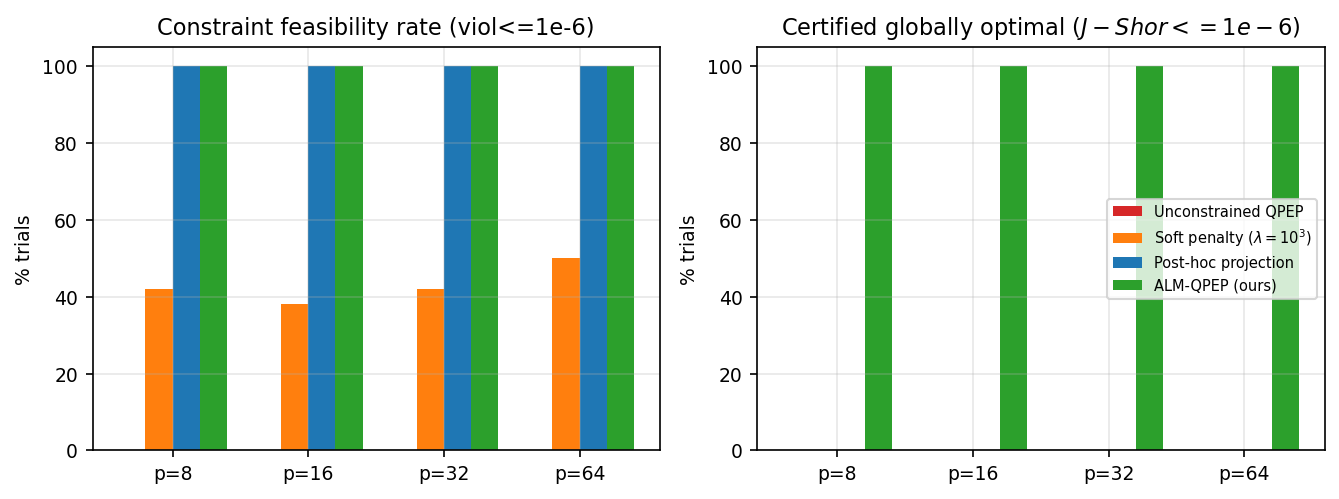
\includegraphics[width=\columnwidth]{fig_main_cert.png}
\caption{Synthetic main sweep: constraint feasibility rate (left) and certified globally optimal rate (right) versus $p$, 50 trials per cell. ALM-QPEP is 100\% feasible and 100\% certified at every $p$; projection is feasible but never certified; the soft penalty is feasible in 38--50\% of trials and never certified.}
\label{fig:app_cert}
\end{figure}

\subsection{Noise, bias and the price of a penalty}\label{app:noise}
Table~\ref{tab:app_noise} fixes $p=16$ and varies the per-point noise $\sigma$ and the vertical bias over four cells. Table~\ref{tab:app_pareto} is a separate 50-trial sweep of the penalty weight $\lambda$ at $p=16$.

\begin{table*}[t]
\centering
\caption{Method $\times$ noise/extrinsic bias at $p=16$ (50 trials per cell; median [IQR]).}
\label{tab:app_noise}
\scriptsize
\setlength{\tabcolsep}{2pt}
\begin{tabular}{@{}llcccccc@{}}
\toprule
cell ($\sigma$ / bias) & method & pen (mm) & rot (deg) & trans (mm) & feasible & certified \\
\midrule
0.000 / 0.000 & Unconstrained QPEP & 0.00 [0.00, 0.00] & 0.00 [0.00, 0.00] & 7.07 [7.07, 7.07] & 100\% & 100\% \\
 & Soft penalty ($\lambda{=}10^3$) & 0.00 [0.00, 0.00] & 0.00 [0.00, 0.00] & 7.07 [7.07, 7.07] & 100\% & 100\% \\
 & Post-hoc projection & 0.00 [0.00, 0.00] & 0.00 [0.00, 0.00] & 7.07 [7.07, 7.07] & 100\% & 100\% \\
 & ALM-QPEP (ours) & 0.00 [0.00, 0.00] & 0.00 [0.00, 0.00] & 7.07 [7.07, 7.07] & 100\% & 100\% \\
\midrule
0.005 / 0.040 & Unconstrained QPEP & 47.52 [38.74, 51.36] & 2.52 [1.58, 3.25] & 45.87 [40.56, 51.75] & 0\% & 0\% \\
 & Soft penalty ($\lambda{=}10^3$) & 0.01 [0.00, 0.03] & 5.10 [3.45, 7.36] & 9.46 [8.10, 11.27] & 24\% & 0\% \\
 & Post-hoc projection & 0.00 [0.00, 0.00] & 2.18 [1.75, 3.16] & 7.79 [7.12, 8.58] & 100\% & 0\% \\
 & ALM-QPEP (ours) & 0.00 [0.00, 0.00] & 2.52 [1.89, 3.33] & 8.46 [7.10, 9.65] & 100\% & 100\% \\
\midrule
0.010 / 0.080 & Unconstrained QPEP & 103.02 [84.69, 110.83] & 5.30 [3.26, 6.70] & 97.90 [88.42, 107.73] & 0\% & 0\% \\
 & Soft penalty ($\lambda{=}10^3$) & 0.00 [0.00, 0.03] & 6.62 [3.70, 9.95] & 13.00 [8.69, 16.87] & 38\% & 0\% \\
 & Post-hoc projection & 0.00 [0.00, 0.00] & 4.16 [2.90, 5.34] & 9.10 [7.34, 10.94] & 100\% & 0\% \\
 & ALM-QPEP (ours) & 0.00 [0.00, 0.00] & 4.17 [2.74, 5.10] & 10.63 [8.17, 12.69] & 100\% & 100\% \\
\midrule
0.020 / 0.120 & Unconstrained QPEP & 198.10 [177.14, 232.79] & 11.50 [7.92, 18.63] & 185.77 [170.38, 215.92] & 0\% & 0\% \\
 & Soft penalty ($\lambda{=}10^3$) & 0.00 [0.00, 0.04] & 11.13 [6.89, 14.36] & 17.01 [10.99, 21.60] & 38\% & 0\% \\
 & Post-hoc projection & 0.00 [0.00, 0.00] & 7.97 [5.45, 11.86] & 12.61 [8.90, 17.11] & 100\% & 0\% \\
 & ALM-QPEP (ours) & 0.00 [0.00, 0.00] & 5.83 [4.49, 7.55] & 13.39 [10.23, 17.43] & 100\% & 100\% \\
\bottomrule
\end{tabular}

\end{table*}

\begin{table}[t]
\centering
\caption{Soft-penalty Pareto at $p=16$ (separate 50-trial sweep; medians).}
\label{tab:app_pareto}
\footnotesize
\begin{tabular}{@{}lcccc@{}}
\toprule
$\lambda$ & pen (mm) & rot (deg) & trans (mm) & feasible \\
\midrule
$10^0$ & 8.72 & 4.34 & 13.32 & 0\% \\
$10^1$ & 2.39 & 5.74 & 11.24 & 0\% \\
$10^2$ & 0.22 & 6.24 & 12.00 & 26\% \\
$10^3$ & 0.00 & 6.61 & 12.53 & 50\% \\
$10^4$ & 0.00 & 6.85 & 12.94 & 48\% \\
\bottomrule
\end{tabular}

\end{table}

Three observations. \textbf{(i) The noise-free cell isolates the injected bias.} With $\sigma=0$ and zero vertical bias, all four methods coincide exactly: 0.00~mm penetration, $0.00^\circ$, and 7.07~mm translation, all 100\% feasible and certified. The 7.07~mm is the fixed 5~mm lateral bias ($\sqrt{5^2+5^2}=7.07$~mm), not a method difference; with no noise the constraints are inactive. \textbf{(ii) Noise and bias separate feasibility from accuracy.} Across the three non-zero cells the unconstrained penetration grows 47.52~$\to$~198.10~mm and it is never feasible; ALM stays at 0.00~mm with 100\% feasibility and certification in all four cells; the soft penalty is feasible in only 24--38\% of the three non-zero cells and is never certified there; projection is 100\% feasible there and never certified. Pose errors are comparable across the three constrained methods at low noise. At the highest cell ALM has the best rotation error ($5.83^\circ$ versus $11.50^\circ$ unconstrained, $11.13^\circ$ soft, $7.97^\circ$ projection) but projection has the best translation (12.61~mm versus ALM 13.39~mm); the differences are within the spread. The robust effect is admissibility and certification, not accuracy. \textbf{(iii) A larger penalty lowers the median penetration but never reaches feasibility.} Table~\ref{tab:app_pareto}: median penetration falls monotonically from 8.72~mm at $\lambda=10^0$ to 0.00~mm at $\lambda=10^3$, at the cost of a rotation error rising from $4.34^\circ$ to $6.85^\circ$ (translation stays flat, 11.24--13.32~mm). Feasibility never exceeds 50\% and is non-monotone (50\% at $\lambda=10^3$, 48\% at $10^4$): the penalty approaches hard feasibility but does not attain it. One seed in 50 falls into a bad local minimum for every $\lambda\ge10$; at $\lambda=10^4$ its rotation error is $132.9^\circ$ and its translation 202.6~mm, and at $\lambda=10^3$ its translation error is 504.6~mm. These outliers are invisible in the medians and are the reason the penalty path cannot be certified.

\begin{figure}[t]
\centering
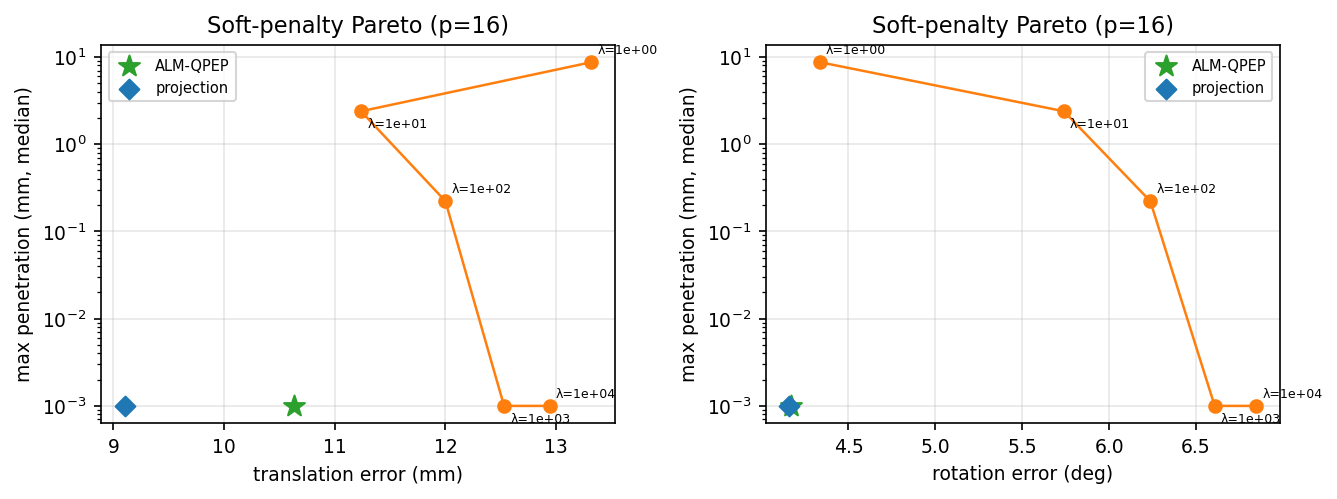
\includegraphics[width=\columnwidth]{fig_pareto.png}
\caption{Soft-penalty Pareto at $p=16$: median maximum penetration versus translation error (left) and versus rotation error (right) as $\lambda$ varies over $10^0$--$10^4$. ALM-QPEP (star) and projection (diamond) are shown for reference.}
\label{fig:app_pareto}
\end{figure}

\begin{figure}[t]
\centering
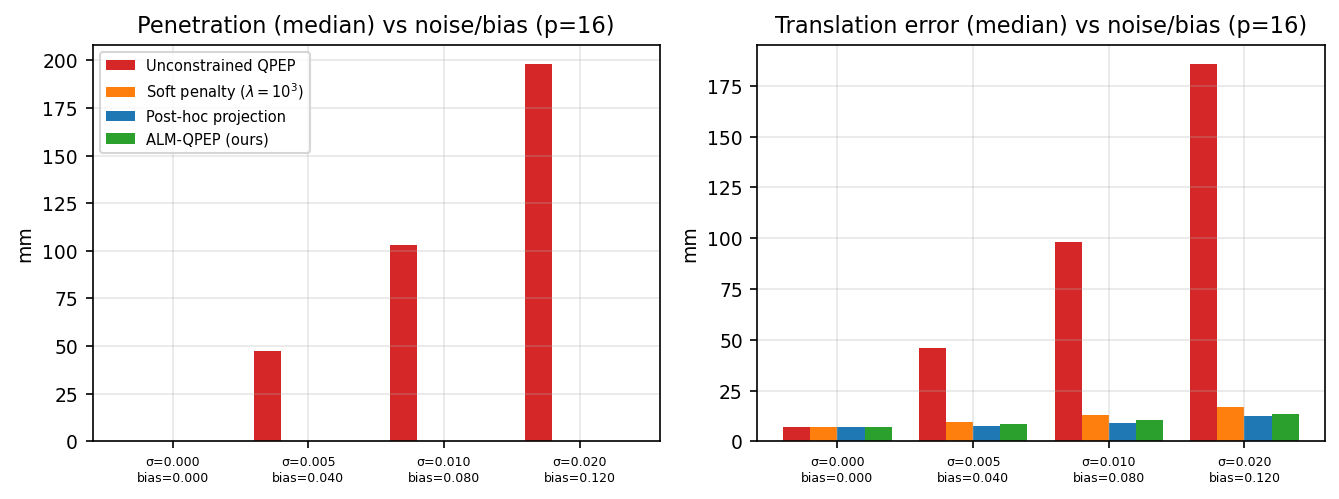
\includegraphics[width=\columnwidth]{fig_noise.png}
\caption{Median penetration (left) and median translation error (right) versus the noise/bias cell at $p=16$ for the four methods.}
\label{fig:app_noise}
\end{figure}

\subsection{Certificate margins, Schur repair and the RLT ablation}\label{app:cert}
\begin{table*}[t]
\centering
\caption{Certificate margins over all 400 synthetic instances (8 cells $\times$ 50).}
\label{tab:app_margins}
\scriptsize
\setlength{\tabcolsep}{3pt}
\begin{tabular}{@{}lcccccc@{}}
\toprule
cell & $n$ & $\max\lambda_2/\lambda_1$ & median $\lambda_2/\lambda_1$ & $\mathrm{Shor}-J_{\rm ALM}$ range & SDP time (mean, ms) \\
\midrule
main $p=8$ & 50 & $1.42\times10^{-9}$ & $9.07\times10^{-11}$ & $[-4.56, 4.29]\times10^{-9}$ & 52.9 \\
main $p=16$ & 50 & $1.03\times10^{-9}$ & $9.47\times10^{-11}$ & $[-3.28, 7.52]\times10^{-9}$ & 57.6 \\
main $p=32$ & 50 & $8.43\times10^{-10}$ & $2.94\times10^{-11}$ & $[-5.66, 5.99]\times10^{-9}$ & 70.0 \\
main $p=64$ & 50 & $1.51\times10^{-9}$ & $9.56\times10^{-11}$ & $[-3.93, 9.41]\times10^{-9}$ & 85.5 \\
noise $0.000/0.000$ & 50 & $5.55\times10^{-10}$ & $1.93\times10^{-11}$ & $[-8.78, 3.57]\times10^{-9}$ & 62.5 \\
noise $0.005/0.040$ & 50 & $8.56\times10^{-10}$ & $7.65\times10^{-11}$ & $[-6.31, 2.67]\times10^{-9}$ & 61.2 \\
noise $0.010/0.080$ & 50 & $1.03\times10^{-9}$ & $9.47\times10^{-11}$ & $[-3.28, 7.52]\times10^{-9}$ & 56.7 \\
noise $0.020/0.120$ & 50 & $1.08\times10^{-9}$ & $2.28\times10^{-11}$ & $[-4.25, 6.82]\times10^{-9}$ & 57.6 \\
\bottomrule
\end{tabular}

\end{table*}

The synthetic relaxation is tight with a wide margin: the largest $\lambda_2/\lambda_1$ over all 400 instances is $1.5\times10^{-9}$, about three orders of magnitude below the $10^{-6}$ threshold, so the 100\% certification rates of Table~\ref{tab:app_main_rates} and of the noise-free cell of Table~\ref{tab:app_noise} are not marginal passes. $\mathrm{Shor}-J_{\rm ALM}$ lies within $\pm10^{-8}$ and changes sign; this is the SCS tolerance, not a theoretical gap, and a rigorous soundness claim needs the dual-feasible repair of Theorem~\ref{thm:cert}. The certificate cost grows from 52.9 to 85.5~ms (means; medians 51~$\to$~84) as $p$ goes from 8 to 64, consistent with a fixed $14\times14$ PSD block and $p$ linear constraints.

\begin{table}[t]
\centering
\caption{The exact Schur bound of Theorem P2-Cert versus the conservative $P$-shift dual repair (6 synthetic instances, $\sigma\in\{0.10,0.20\}$, $p=16$).}
\label{tab:app_schur}
\scriptsize
\setlength{\tabcolsep}{3pt}
\begin{tabular}{@{}ccccc@{}}
\toprule
$\sigma$ & seed & $J$ & $J-\text{dual repair}$ & $J-\text{Schur}$ \\
\midrule
0.10 & 0 & 9.0579e-01 & $2.00\times10^{-8}$ & $5.59\times10^{-12}$ \\
0.10 & 1 & 6.8500e-01 & $2.00\times10^{-8}$ & $-6.69\times10^{-13}$ \\
0.10 & 2 & 4.3643e-01 & $2.00\times10^{-8}$ & $5.31\times10^{-11}$ \\
0.20 & 0 & 3.2392e+00 & $2.04\times10^{-8}$ & $4.22\times10^{-10}$ \\
0.20 & 1 & 3.1128e+00 & $2.00\times10^{-8}$ & $3.81\times10^{-11}$ \\
0.20 & 2 & 3.0309e+00 & $2.01\times10^{-8}$ & $6.21\times10^{-11}$ \\
\bottomrule
\end{tabular}

\end{table}

Both bounds are sound; the 13$\times$13 translation Schur complement is the tighter one by about four orders of magnitude. The $P$-shift repair pays a $2c$ loss from bounding $\|\mathbf t\|$, so its gap is pinned at $2\delta_{\rm round}\approx2\times10^{-8}$, while the Schur bound needs no $\|\mathbf t\|$ bound and leaves $5.6\times10^{-12}$--$4.2\times10^{-10}$ on five of the six rows. The sixth row records $J-d_{\rm sound}=-6.7\times10^{-13}$: that is the size of the floating-point margin $\delta_{\rm round}\sim10^{-12}\|\mathbf S_{10}\|_F$ which Theorem P2-Cert subtracts, i.e.\ a rounding residual at the level of the certified margin, not a structural overshoot---the paper reports the raw difference and does not round it to ``positive''. Consequence: \texttt{rigorous\_schur} is the bound of record; the $P$-shift \texttt{repair\_dual} value is retained only as a conservative fallback (and is the value quoted in the synthetic 16/16 result of App.~\ref{app:baselines}, which predates the Schur path). All six rows are case~A (the $3\times3$ translation block is positive definite), so the tighter branch of the theorem is the one exercised.

\begin{table*}[t]
\centering
\caption{Zero-dimensional RLT ablation at four noise levels (4 seeds per cell).}
\label{tab:app_rlt}
\scriptsize
\setlength{\tabcolsep}{2pt}
\begin{tabular}{@{}lcccccccc@{}}
\toprule
$\sigma$ / bias & $n$ & base cert & +RLT cert & median abs gap, base & median abs gap, +RLT & base time (s) & RLT time (s) \\
\midrule
0.02 / 0.10 & 4 & 4/4 & 4/4 & $1.6\times10^{-10}$ & $8.1\times10^{-11}$ & 0.05 & 0.15 \\
0.05 / 0.20 & 4 & 4/4 & 4/4 & $1.7\times10^{-9}$ & $9.4\times10^{-10}$ & 0.05 & 0.14 \\
0.10 / 0.30 & 4 & 1/4 & 2/4 & $4.2\times10^{-4}$ & $2.9\times10^{-4}$ & 1.59 & 0.85 \\
0.20 / 0.40 & 4 & 0/4 & 0/4 & $8.6\times10^{-3}$ & $7.8\times10^{-3}$ & 1.62 & 2.40 \\
\bottomrule
\end{tabular}

\end{table*}

The zero-dimensional RLT cuts $g_ig_j\ge0$ (136 rows at $p=16$) help only when the base gap is small enough for a modest tightening to cross the threshold, and nowhere else:
\begin{itemize}
\item At $\sigma=0.02$ and $0.05$ the base certificate is already 4/4, so RLT changes nothing.
\item At $\sigma=0.10$ the base certifies 1/4; RLT certifies 2/4. The gain is one seed whose gap drops from $2.4\times10^{-4}$ to $7.6\times10^{-12}$; the already-certified seed stays certified, and the two remaining seeds stay uncertified with gaps of $3.1\times10^{-3}$ and $5.8\times10^{-4}$.
\item At $\sigma=0.20$ both methods certify 0/4. RLT reduces the per-seed gap by 10--17\% (median $8.6\times10^{-3}\to7.8\times10^{-3}$), which is still about four orders of magnitude above the $10^{-6}$ tolerance.
\item The RLT certificate costs about $3\times$ the base SDP on the low-noise cells (0.05~$\to$~0.15~s) and 0.1--2.6~s per instance on the high-noise cells, where both solves are inaccurate.
\end{itemize}
The failures at $\sigma=0.10$ and $0.20$ show that zero-dimensional RLT does not close the gap; the sound higher-order bound-RLT family does, on the synthetic cells (App.~\ref{app:baselines}) and on real data (App.~\ref{app:real}).

\textbf{Which inner root count applies.} All synthetic cells above use a PnP-type base, i.e.\ Type~I of Theorem~\ref{thm:spectrum}: the reduced matrix is rank-deficient (rank 9 at $\sigma=0.01$, rank 8 at $\sigma=0$) but the inner KKT system still has $N_{\mathbb C}=40$ complex projective roots with the generic 15-monomial grevlex staircase, because the shift $\mathbf M\mapsto\mathbf M+\alpha\mathbf I$ changes $f$ only by $\alpha(\mathbf q^\top\mathbf q)^2$ and leaves every critical point in place; the homotopy then finds 16--18 \emph{real} roots per instance, the expected Type-I picture. The compact families differ: an isotropic 3D--3D (Horn) base with $k$ active plane constraints sharing one normal collapses to $N_{\mathbb C}=4/12/16$ for $k=0/1/\ge2$ (the Hopf ruled line $\mathcal L_{\mathbf n}$ is an excess component that must be saturated), to $32$ for two distinct normals, and to $40$ for an anisotropic/PnP base with any plane. The implementation ships the 40-root unsaturated template for the generic and PnP cases, and solves the isotropic single-plane family with the 162-path homotopy plus a multistart fallback; the $16\times16$ saturated action matrix is not built as a numeric template, and the $4/12/16$ spectrum is validated numerically in canonical form (App.~\ref{app:deriv}). The exact-enumeration timings in App.~\ref{app:baselines} are measured on the Type-I instances.

\subsection{Real-data layer results}\label{app:real}
\begin{table*}[t]
\centering
\caption{Per-cell rigorous certification ($p=16$, $n=90/72/84$, bit-identical ALM replay). ``cert'' = ALM feasible and $J-d_{\rm sound}\le10^{-6}$ with $d_{\rm sound}$ a proven lower bound; Wilson 95\% CIs; zero-dimensional RLT adds 136 rows ($p:16\to152$), bound-RLT adds 320 ($16\to336$). ``One-sided'' is the same $J-\mathrm{Shor}\le10^{-6}$ rule applied to the solver value in the replay.}
\label{tab:rigorous_full}
\scriptsize
\setlength{\tabcolsep}{2.5pt}
\begin{tabular}{@{}llp{1.9cm}ccccp{5.0cm}c@{}}
\toprule
Dataset & $n$ & Cut family & Rigorous Schur & 95\% CI & Rigorous $P$-shift & 95\% CI & Schur gap (min / median / max) & One-sided \\
\midrule
\multirow{3}{*}{LM} & \multirow{3}{*}{90} & base & \textbf{22 (24.4\%)} & [16.7, 34.2] & 23 (25.6\%) & [17.7, 35.4] & $4.0{\times}10^{-12}$ / $9.1{\times}10^{-6}$ / $4.0{\times}10^{-4}$ & 25 \\
 & & zero-dim RLT & 19 (21.1\%) & [14.0, 30.6] & 18 (20.0\%) & [13.0, 29.4] & $9.3{\times}10^{-12}$ / $1.6{\times}10^{-5}$ / $2.3{\times}10^{-1}$ & 35 \\
 & & bound-RLT & \textbf{46 (51.1\%)} & [41.0, 61.2] & 43 (47.8\%) & [37.8, 58.0] & $4.0{\times}10^{-12}$ / $3.4{\times}10^{-7}$ / $2.8{\times}10^{-1}$ & 61 \\
\midrule
\multirow{3}{*}{LM-O} & \multirow{3}{*}{72} & base & \textbf{11 (15.3\%)} & [8.8, 25.3] & 11 (15.3\%) & [8.8, 25.3] & $1.7{\times}10^{-11}$ / $1.6{\times}10^{-5}$ / $2.6{\times}10^{-4}$ & 19 \\
 & & zero-dim RLT & 6 (8.3\%) & [3.9, 17.0] & 6 (8.3\%) & [3.9, 17.0] & $3.2{\times}10^{-11}$ / $6.4{\times}10^{-5}$ / $3.3$ & 19 \\
 & & bound-RLT & \textbf{30 (41.7\%)} & [31.0, 53.2] & 24 (33.3\%) & [23.5, 44.8] & $5.6{\times}10^{-12}$ / $2.1{\times}10^{-6}$ / $9.4{\times}10^{-2}$ & 45 \\
\midrule
\multirow{3}{*}{YCB-V} & \multirow{3}{*}{84} & base & \textbf{11 (13.1\%)} & [7.5, 21.9] & 10 (11.9\%) & [6.6, 20.5] & $1.0{\times}10^{-11}$ / $2.1{\times}10^{-5}$ / $4.0{\times}10^{-4}$ & 17 \\
 & & zero-dim RLT & 6 (7.1\%) & [3.3, 14.7] & 6 (7.1\%) & [3.3, 14.7] & $1.0{\times}10^{-11}$ / $3.8{\times}10^{-5}$ / $1.1$ & 11 \\
 & & bound-RLT & \textbf{20 (23.8\%)} & [16.0, 33.9] & 19 (22.6\%) & [15.0, 32.6] & $4.1{\times}10^{-12}$ / $1.3{\times}10^{-5}$ / $3.0$ & 31 \\
\bottomrule
\end{tabular}
\end{table*}

\begin{figure*}[t]
\centering
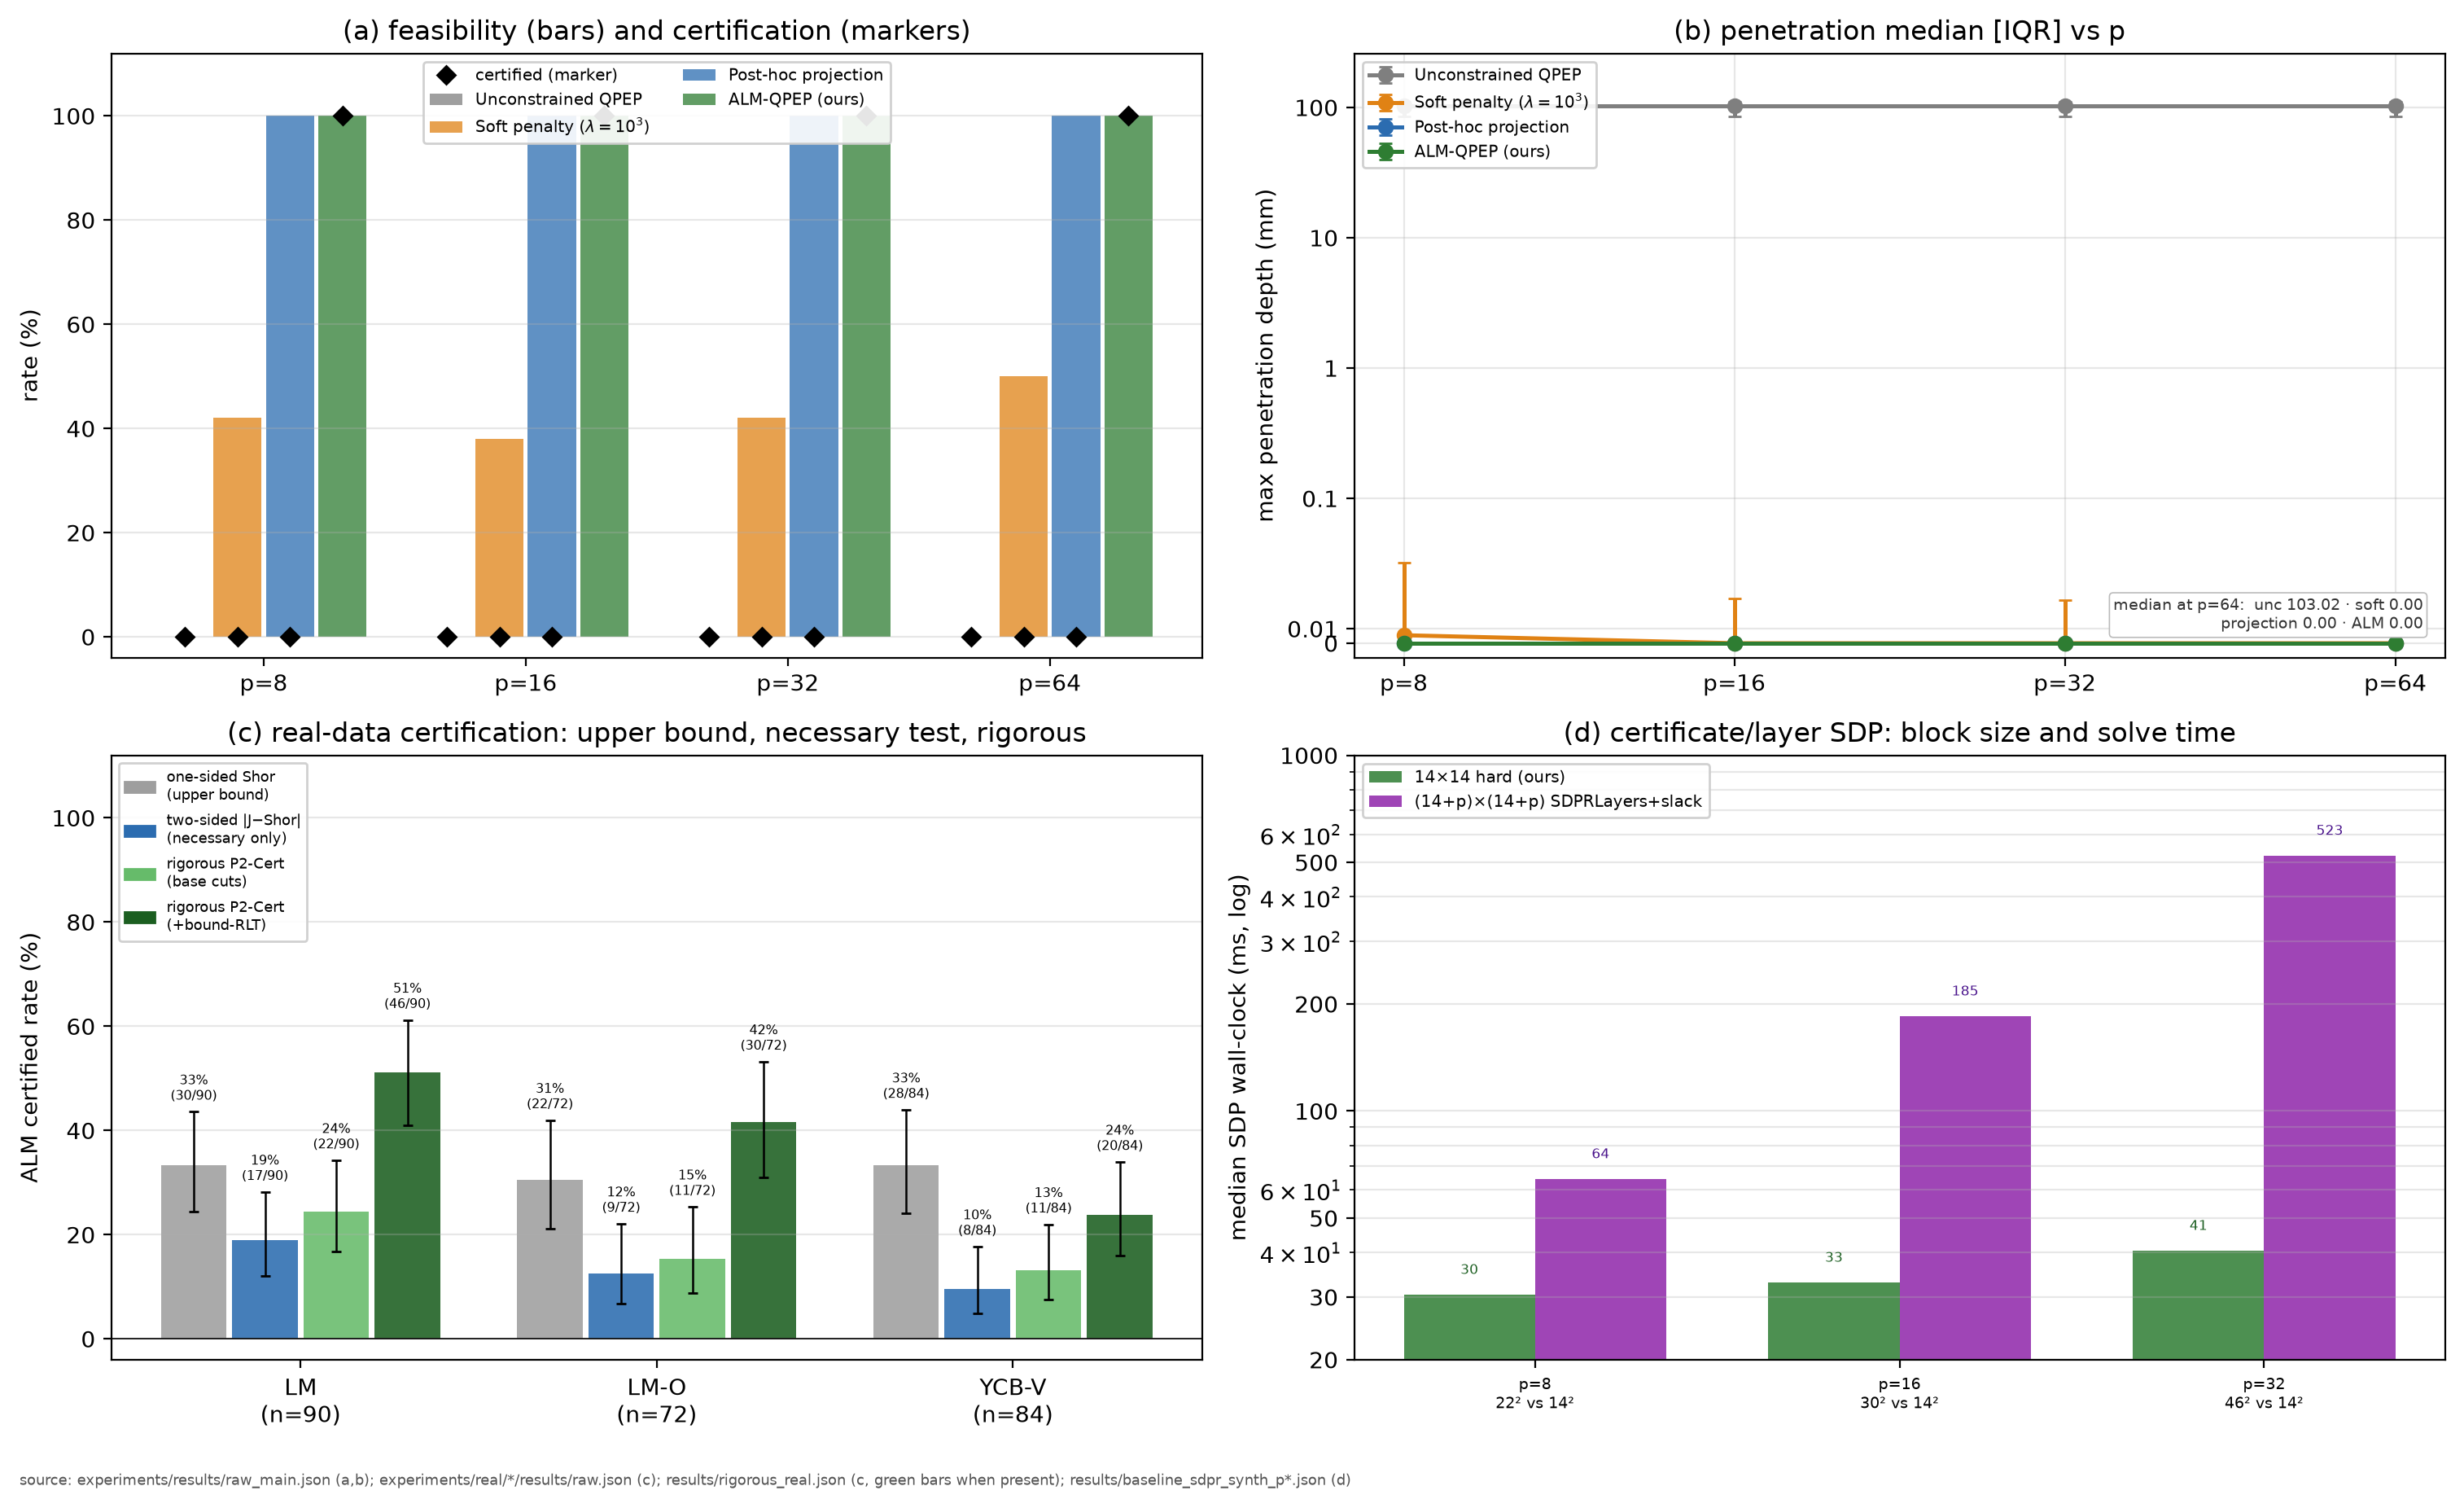
\includegraphics[width=\textwidth]{fig_p2_overview.png}
\caption{Overview. (a)~Feasibility (bars) and certification (filled diamonds) versus $p$ for the four methods, 50 trials per cell. (b)~Maximum penetration depth, median [IQR], versus $p$ on a symlog axis (projection and ALM coincide at 0.00). (c)~Real-data ALM certification at $n=90/72/84$: the one-sided Shor flag (an upper bound, grey), the two-sided $|J-\mathrm{Shor}|$ test (necessary only, blue) and the rigorous P2-Cert bound (green), with 95\% Wilson intervals.}
\label{fig:overview}
\end{figure*}

\begin{table*}[t]
\centering
\caption{Real-data layer experiment ($p=16$, ground-truth-projected correspondences; $n=90/72/84$).}
\label{tab:app_real}
\scriptsize
\setlength{\tabcolsep}{3pt}
\begin{tabular}{@{}llccccccc@{}}
\toprule
dataset & $n$ & method & pen (mm) & rot (deg) & trans (mm) & feasible & cert one-sided (upper bound) & cert two-sided (necessary) \\
\midrule
LINEMOD & 90 & Unconstrained QPEP & 11.26 & 2.08 & 35.63 & 13.3\% & 13.3\% & 8.9\% \\
 & & Soft penalty ($\lambda{=}10^3$) & 0.00 & 2.13 & 39.81 & 88.9\% & 26.7\% & 16.7\% \\
 & & Post-hoc projection & 0.00 & 2.05 & 30.80 & 100\% & 15.6\% & 10.0\% \\
 & & \textbf{ALM-QPEP (ours)} & \textbf{0.00} & \textbf{1.97} & \textbf{37.66} & \textbf{100\%} & \textbf{33.3\%} & \textbf{18.9\%} \\
\midrule
LM-O & 72 & Unconstrained QPEP & 14.93 & 2.07 & 34.69 & 6.9\% & 6.9\% & 6.9\% \\
 & & Soft penalty ($\lambda{=}10^3$) & 0.00 & 1.90 & 39.91 & 91.7\% & 26.4\% & 9.7\% \\
 & & Post-hoc projection & 0.00 & 2.04 & 31.29 & 100\% & 8.3\% & 6.9\% \\
 & & \textbf{ALM-QPEP (ours)} & \textbf{0.00} & \textbf{1.99} & \textbf{38.14} & \textbf{100\%} & \textbf{30.6\%} & \textbf{12.5\%} \\
\midrule
YCB-Video & 84 & Unconstrained QPEP & 14.09 & 1.08 & 17.33 & 6.0\% & 6.0\% & 3.6\% \\
 & & Soft penalty ($\lambda{=}10^3$) & 0.00 & 1.40 & 29.38 & 90.5\% & 21.4\% & 7.1\% \\
 & & Post-hoc projection & 0.00 & 1.08 & 8.93 & 100\% & 7.1\% & 4.8\% \\
 & & \textbf{ALM-QPEP (ours)} & \textbf{0.00} & \textbf{1.11} & \textbf{25.18} & \textbf{100\%} & \textbf{33.3\%} & \textbf{9.5\%} \\
\bottomrule
\end{tabular}

\end{table*}

Six observations. \textbf{(i) The unconstrained solve is infeasible on real object/table geometry.} It violates feasibility in 86.7\% (LM), 93.1\% (LM-O) and 94.0\% (YCB-Video), with median penetration 11.26/14.93/14.09~mm. ALM is 100\% feasible with 0.00~mm penetration on all three datasets; the soft penalty is feasible in 88.9\%/91.7\%/90.5\%. Projection is also 100\% feasible. \textbf{(ii) Constraints buy admissibility, not accuracy.} All four methods are within $1.1$--$2.1^\circ$ rotation and 9--40~mm translation. ALM is not more accurate than projection (translation 37.66 vs 30.80~mm on LM, 38.14 vs 31.29~mm on LM-O, 25.18 vs 8.93~mm on YCB-Video). \textbf{(iii) Real certification is upper-bounded and dataset-dependent.} The one-sided ALM rates are 33.3\% [24.5,43.6] (LM), 30.6\% [21.1,42.0] (LM-O), 33.3\% [24.2,43.9] (YCB-Video); the two-sided rates are 18.9\%, 12.5\%, 9.5\%. The zero-dimensional RLT cuts do \textbf{not} give a reproducible real gain: LM 33.3~$\to$~31.1 (McNemar $p=0.85$), LM-O 30.6~$\to$~33.3 ($p=0.86$), YCB 33.3~$\to$~23.8 ($p=0.15$, worse); on the two-sided test RLT is worse everywhere (18.9~$\to$~14.4, 12.5~$\to$~4.2, 9.5~$\to$~6.0). Zero-dimensional RLT therefore does not improve certification on real data. \textbf{(iv) The stored real-data certificate flag is one-sided.} It tests \texttt{feasible and J - Shor <= 1e-6}, does not record $\lambda_2/\lambda_1$ or the SDP solution state, and accepts negative gaps. On the scaled runs 18--26\% of base ALM rows have negative gaps, and the two-sided rates are 9.5--18.9\%. The rates in Table~\ref{tab:app_real} are therefore \textbf{upper bounds}; the rigorous replacements are in Table~\ref{tab:rigorous}. \textbf{(v) Rigorous certification and the one positive RLT result.} Table~\ref{tab:rigorous} replaces both flags by \emph{proven} lower bounds: \texttt{rigorous\_schur} (the 13-dimensional translation Schur complement, the bound of record) and, as a conservative fallback, the $P$-shift \texttt{repair\_dual} value. The counts verify the sandwich on every dataset (one-sided $\ge$ rigorous $\ge$ two-sided). \textbf{(vi) Why the LM-O pure-plane rows need cross-direction cuts.} See App.~\ref{app:lmo}.

Five readings. \emph{(a) The rigorous rates are much lower than the one-sided upper bounds}---LM 24.4\% vs 33.3\%, LM-O 15.3\% vs 30.6\%, YCB-Video 13.1\% vs 33.3\%---and consistently above the two-sided necessary test (18.9/12.5/9.5). The sandwich is ordered as it must be, and the gap between the upper bound and the sound rate (9--20 percentage points) is the size of the numerical illusion that the one-sided flag was reporting. \emph{(b) The uncertified rows are genuinely slack, not numerical failures.} The Schur gap is non-negative on every one of the 738 replay rows (3 cut families $\times$ 246 instances; 0 negative gaps, minimum $4.0\times10^{-12}$--$1.7\times10^{-11}$, at the rounding floor), and the median gap on the base configuration is $9.1\times10^{-6}$/$1.6\times10^{-5}$/$2.1\times10^{-5}$---9--21$\times$ the $10^{-6}$ tolerance. Tightness, not round-off, is the binding limitation on real data. \emph{(c) The Schur bound and the $P$-shift bound are within 1--2 rows on real data} (22 vs 23, 11 vs 11, 11 vs 10), unlike the four-orders-of-magnitude separation on the synthetic high-noise cells (Table~\ref{tab:app_schur}); per row the Schur value is the tighter of the two on 82/90, 68/72 and 78/84 base rows, and all 738 replay rows are case~A ($\tilde{\mathbf H}_{tt}\succ0$, maximum condition number 1668), so the tight branch of Theorem P2-Cert is the one exercised and no row needs the $R_t$ ball. The reason is the previous point: the $2\delta_{\rm round}\approx2\times10^{-8}$ cost of the $P$-shift is irrelevant when the gaps are $\ge10^{-5}$. We still report the Schur value as the bound of record and the $P$-shift value as a fallback, because the ordering is the opposite (Schur tighter) wherever the gap reaches the rounding floor. \emph{(d) The one-sided count is not reproducible across SDP re-solves.} On the identical instances (ALM $J$ bit-identical), the replay re-solves the SDP at \texttt{eps=1e-9}, 50k iterations instead of the stored run's 20k, and its value differs by a median of $2.3\times10^{-8}$ and a maximum of $3.7\times10^{-2}$; applying the \emph{same} $J-\mathrm{Shor}\le10^{-6}$ rule to the replay's value gives 25/90, 19/72, 17/84 where the stored table reports 30/90, 22/72, 28/84. A test whose own count moves by 5--11 rows between solves is not a certificate, which is why the paper retires it as an upper bound only. \emph{(e) Sound bound-RLT is a positive result, and the earlier negative conclusion came from the unsound value.} Compared with the base configuration, the sound higher-order bound-RLT family raises rigorous certification from 22~$\to$~46 (LM), 11~$\to$~30 (LM-O), 11~$\to$~20 (YCB-Video) on the Schur bound---$+26.7/+26.4/+10.7$ percentage points---with McNemar $p=8.4\times10^{-6}$, $1.6\times10^{-4}$, $3.5\times10^{-2}$ (paired flags; $0\to1$ flips 27/22/12 against $1\to0$ flips 3/3/3). On the more conservative $P$-shift bound the same counts are 23~$\to$~43, 11~$\to$~24, 10~$\to$~19 ($+22.2/+18.1/+10.7$~pp; the paired test is reported on the Schur value only). The zero-dimensional family is null or negative under the same sound rule (Schur 22~$\to$~19, 11~$\to$~6, 11~$\to$~6; $p=0.45/0.063/0.063$). On the \emph{stored values} the zero-dimensional RLT appeared to help on LM-O (22~$\to$~24) only because it pushed values above $J$ on 22/72 rows; with a sound bound that apparent gain disappears, while the bound-RLT family---judged a failure when read through the unsound flag---is the one that actually closes gaps.

\subsection{LM-O depth and tilt augmentation}\label{app:lmo}
The structural diagnosis of Theorem~\ref{thm:cert} says that when every active constraint shares the table normal, the RLT products constrain only $\mathbf n^\top\mathbf t$, leaving a rank-2 pseudo-mixture admissible, and that positive-depth and tilt-cone rows add the cross-direction blocks that cut it. Table~\ref{tab:app_lmo} tests that prediction on the six LM-O rows with the largest Schur gap under the base configuration (all frame 000002, objects 5/8/12, bias 20/30~px; 61 of 72 base rows are uncertified).

\begin{table*}[t]
\centering
\caption{LM-O depth+tilt augmentation, before $\to$ after (6 worst base-uncertified rows).}
\label{tab:app_lmo}
\scriptsize
\setlength{\tabcolsep}{4pt}
\begin{tabular}{@{}lccccc@{}}
\toprule
row (frame/img/obj/bias) & gap, base & gap, bound-RLT (no aug.) & gap, aug.+base & gap, aug.+bound-RLT & certified after \\
\midrule
000002/1/8/30 & $2.56\times10^{-4}$ & $1.45\times10^{-4}$ & $2.54\times10^{-4}$ & $9.0\times10^{-12}$ & yes \\
000002/0/8/30 & $2.56\times10^{-4}$ & $2.00\times10^{-4}$ & $2.37\times10^{-4}$ & $5.2\times10^{-11}$ & yes \\
000002/1/5/30 & $1.78\times10^{-4}$ & $3.54\times10^{-5}$ & $1.77\times10^{-4}$ & $1.0\times10^{-11}$ & yes \\
000002/0/5/30 & $1.15\times10^{-4}$ & $1.0\times10^{-10}$ & $1.15\times10^{-4}$ & $9.9\times10^{-11}$ & yes \\
000002/0/8/20 & $1.02\times10^{-4}$ & $6.17\times10^{-5}$ & $1.02\times10^{-4}$ & $1.9\times10^{-11}$ & yes \\
000002/0/12/30 & $1.00\times10^{-4}$ & $9.37\times10^{-5}$ & $9.9\times10^{-5}$ & $6.0\times10^{-11}$ & yes \\
\bottomrule
\end{tabular}

\end{table*}

The prediction holds in a specific and checkable form. (a) The augmentation does not change the answer: $|\Delta J|\le7.4\times10^{-15}$ and ALM's pose already satisfies the added rows (minimum depth 0.85--0.88~m $\gg z_{\min}=0.02$~m; upright 0.998--0.999 $\ge\cos12^\circ=0.978$), so the certificate is for a problem with the same optimum, not for a different one. (b) The extra rows \emph{alone} do nothing: base cuts on the augmented problem still fail on all six (gaps $9.9\times10^{-5}$--$2.5\times10^{-4}$, essentially unchanged). (c) With bound-RLT on the augmented problem all six certify, at gaps $9\times10^{-12}$--$1.0\times10^{-10}$; without the augmentation, bound-RLT alone certifies only 1 of the 6 (gap $1.0\times10^{-10}$ for that one, $3.5\times10^{-5}$--$2.0\times10^{-4}$ for the rest). So it is the \emph{cross-direction RLT products} $g_{\rm plane}g_{\rm depth}$ and $g_{\rm plane}g_{\rm tilt}$ that carry the gain, exactly as the theorem argues, and the depth/tilt rows are the enabler rather than the cure. These are 6 of the 61 uncertified LM-O rows, selected as the worst: a mechanism check rather than a dataset-level rate, the latter remaining those of Table~\ref{tab:rigorous}.

\subsection{Baselines and exact enumeration}\label{app:baselines}
\textbf{Measured in this round.} All numbers are layer-level and were produced on a shared login node; absolute timings drift with load and are used only for relative comparison.

\begin{itemize}
\item \textbf{Exact QPEP inner enumeration, end-to-end through ALM.} On 8 ALM trials at $p\in\{8,16,64\}$ (seeds 0--3 at $p=16$, seeds 0--1 at $p=8,64$), the exact 162-path total-degree enumerator and the default 6-start multistart return the same objective to $\max|\Delta J|=1.8\times10^{-12}$, the same pose to $\max\|\Delta\mathbf q\|=7.9\times10^{-10}$, the same feasibility (max violation $7.6\times10^{-11}$) and the same outer iteration count on 7/8 trials (the remaining $p=64$ trial stops one iteration earlier). Completeness is conditional and measured: 89/114 enumerations (78.1\%) found the generic 40 finite projective roots, while 25 (21.9\%) lost a homotopy path and fell back to a 64-start BFGS; every one of the 114 probed enumerations had a fresh 64-start BFGS reach the same global minimum. At $\sigma=0.01$ the ALM active-set matrix is full rank (10/10, min eigenvalue $8.2\times10^{-4}$) while the unconstrained $\mathbf M^{\rm red}_{\mathcal A}$ is rank 9; the noise-free matrix is rank 8 with 16--18 real roots. The 25 fallbacks are therefore homotopy path loss, not rank deficiency. The exact inner costs 5.0--15.9~s per pose against 0.12--0.28~s for multistart (37--64$\times$, median $47\times$); a hybrid schedule (exact enumeration every third outer iteration) cuts that to 2.1--4.0~s at the same objective. It therefore buys a correctness/global-optimality check of the inner block at a fixed active set, not a competitive inner solver; the default remains multistart.
\item \textbf{Enumeration-cost update (measured separately, not rescaled).} The 37--64$\times$ ratios above were measured with the pre-optimisation enumerator (one 162-path enumeration $\approx649$~ms on average). A later row of the same code replaced the three-operand \texttt{einsum} that forms $\mathbf J^\top\mathbf M\mathbf J$ by two batched BLAS products ($\mathbf M\mathbf J$ then $\mathbf J^\top(\mathbf M\mathbf J)$, mathematically identical), taking one enumeration from 0.488~s to 0.168~s (2.92$\times$, 356~$\to$~1077 paths/s) with exact parity on 15 cases (same root counts, same finite projective counts, $\max|\Delta f|=3.3\times10^{-16}$) and the same number of batch evaluations (median 470). We keep the directly measured 37--64$\times$ figure for the end-to-end ALM comparison and report the 2.92$\times$ as an isolated inner-loop speedup. A rejected variant (early culling of divergent paths, \texttt{div\_tol} $10^3$--$10^2$) gained nothing at $10^3$ and lost roots at $10^2$, so it was reverted.
\item \textbf{SCP baseline (dQP + local linearisation).} On the synthetic main cells ($p=8/16/32$, 50 trials each) SCP is 100\% feasible, matches ALM's pose error to the printed precision ($p=16$: 0.00~mm / $4.17^\circ$ / 10.63~mm) and its output passes the same $14\times14$ certificate test in 98\% of trials against ALM's 100\%; it is faster in this implementation (median 130--142~ms versus 218--239~ms) with about 90\% of its wall clock in the SOCP. On the pressure cell ($\sigma=0.020$, bias 0.120, 20 trials) SCP certifies 85\% against ALM's 100\%. All six SCP failures start from a cheirality-mirror unconstrained solution and are not rescued by two extra perturbed starts. The differentiators we claim are therefore the mirror-initialisation robustness and the $p$-independent complexity argument, not per-instance accuracy; SCP is a mandatory strong baseline and is reported as such.
\item \textbf{Sound higher-order RLT (synthetic).} A sound bound-RLT family combined with \texttt{repair\_dual} certifies all 16 synthetic noise instances (9/16 before), with maximum rigorous gap $2.28\times10^{-8}$ and median certificate time 0.036~s $\to$ 0.180~s. The gains are concentrated where zero-dimensional cuts alone failed ($\sigma=0.10$: 1/4~$\to$~4/4; $\sigma=0.20$: 0/4~$\to$~4/4).
\item \textbf{Rigorous real-data certification and the bound-RLT result.} The stored one-sided flags are replaced by proven lower bounds on all three datasets (Table~\ref{tab:rigorous}). Base configuration: rigorous Schur 22/90 (24.4\%), 11/72 (15.3\%), 11/84 (13.1\%)---all below the one-sided upper bounds (33.3/30.6/33.3\%) and above the two-sided necessary tests (18.9/12.5/9.5\%). The Schur bound is non-negative on all 738 replay rows (min $4.0\times10^{-12}$), so the failure mode is slack: the median base gap is $9.1\times10^{-6}$/$1.6\times10^{-5}$/$2.1\times10^{-5}$, 9--21$\times$ the tolerance. Adding the sound bound-RLT family raises the rigorous rate to 46/90 (51.1\%), 30/72 (41.7\%), 20/84 (23.8\%), i.e.\ $+26.7/+26.4/+10.7$~pp on the Schur bound ($+22.2/+18.1/+10.7$~pp on the $P$-shift counts), paired McNemar $p=8.4\times10^{-6}$, $1.6\times10^{-4}$, $3.5\times10^{-2}$, at a 0.9--1.5$\times$ SDP cost and a 0.20--0.36~ms Schur repair. The zero-dimensional RLT family stays null or negative under the same sound rule (Schur 22~$\to$~19, 11~$\to$~6, 11~$\to$~6; $p=0.45/0.063/0.063$). The reading is therefore that zero-dimensional RLT does not improve certification, while sound bound-RLT does.
\end{itemize}

\textbf{Further experiments.} Learned and remaining convex-layer baselines (SDPRLayers unconstrained and with $p$ slacks, Theseus), end-to-end training on the T1-network, T2 and T3 protocols, backward-pass and latency decomposition, and real-data scale-up beyond $n=90/72/84$ are the natural extensions of this study. The experiments above use the research implementation under \texttt{experiments/code/}; all result files, the aggregation script and the figure script are under \texttt{experiments/results/}, and the verification scripts and outputs are under \texttt{verify/}.

\subsection{Danskin gluing lemma}\label{app:danskin}
The ALM inner problem is solved with a frozen active set, but the outer objective must be differentiable across the surfaces where that set changes. The following lemma supplies the missing $C^1$ step; it is used in Sec.~\ref{sec:alm} and in the multi-start inner solver.
\begin{lemma}[Global $C^1$ gluing of the eliminated ALM objective]\label{lem:danskin}
Fix $\boldsymbol\mu\in\mathbb{R}^p_{\ge0}$ and $\rho>0$, let $\mathcal L_\rho$ be \eqref{eq:alm}, and assume $J_\theta(\mathbf q,\mathbf t)=\mathbf t^\top\mathbf G_0\mathbf t+2\boldsymbol\ell(\mathbf q)^\top\mathbf t+\alpha(\mathbf q)$ with $\mathbf G_0\succeq\lambda_{\min}(\mathbf G_0)\mathbf I_3\succ0$ and every $g_j$ affine in $\mathbf t$. Define $\phi_\rho(\mathbf q):=\min_{\mathbf t\in\mathbb{R}^3}\mathcal L_\rho(\mathbf q,\mathbf t,\boldsymbol\mu)$ and $\mathbf t^\star(\mathbf q):=\argmin_{\mathbf t}\mathcal L_\rho(\mathbf q,\mathbf t,\boldsymbol\mu)$. Then:
(i) for every $\mathbf q\in\mathbb S^3$, $\mathbf t\mapsto\mathcal L_\rho(\mathbf q,\mathbf t,\boldsymbol\mu)$ is $C^1$ and $2\lambda_{\min}(\mathbf G_0)$-strongly convex, so $\mathbf t^\star(\mathbf q)$ is unique;
(ii) $\mathbf t^\star$ is Lipschitz on $\mathbb S^3$ and $\mathbf t^\star(\mathbb S^3)$ lies in a fixed compact ball $\overline{B(\mathbf 0,R)}$;
(iii) $\phi_\rho\in C^1(\mathbb S^3)$ across active-set switching surfaces, with $\nabla_{E,\mathbf q}\phi_\rho(\mathbf q)=\nabla_{E,\mathbf q}\mathcal L_\rho(\mathbf q,\mathbf t^\star(\mathbf q),\boldsymbol\mu)$ and $\operatorname{grad}_{\mathbb S^3}\phi_\rho=(\mathbf I_4-\mathbf q\mathbf q^\top)\nabla_{E,\mathbf q}\phi_\rho$;
(iv) on each open cell of constant active pattern, $\phi_\rho$ is $C^\infty$ and equals the $10$-dimensional quartic $\mathbf v_2^\top\mathbf M_{\mathcal A}\mathbf v_2+\kappa_{\mathcal A}$ of Theorem~\ref{thm:dim}.
\end{lemma}
\begin{proof}
(i) The scalar hinge $\varphi(u)=\tfrac12[u]_+^2$ is convex and $C^1$ with $\varphi'(u)=[u]_+$, and $u_j(\mathbf q,\mathbf t)=\mu_j+\rho g_j$ is affine in $\mathbf t$; hence each penalty term is convex and $C^1$ in $\mathbf t$. Adding $\mathbf t^\top\mathbf G_0\mathbf t$ with $2\mathbf G_0\succeq2\lambda_{\min}(\mathbf G_0)\mathbf I_3$ gives strong convexity, hence a unique minimiser.

(ii) First-order optimality at $\mathbf t^\star(\mathbf q)$ and strong monotonicity give
\begin{equation}
\begin{aligned}
2\lambda_{\min}(\mathbf G_0)&\|\mathbf t^\star\|_2^2
\le\big(\nabla_{\mathbf t}\mathcal L_\rho(\mathbf q,\mathbf t^\star)-\nabla_{\mathbf t}\mathcal L_\rho(\mathbf q,\mathbf 0)\big)^\top\mathbf t^\star\\
&=-\nabla_{\mathbf t}\mathcal L_\rho(\mathbf q,\mathbf 0)^\top\mathbf t^\star
\le\|\nabla_{\mathbf t}\mathcal L_\rho(\mathbf q,\mathbf 0)\|_2\|\mathbf t^\star\|_2 .
\end{aligned}
\end{equation}
Since $\mathbf q\mapsto\nabla_{\mathbf t}\mathcal L_\rho(\mathbf q,\mathbf 0)$ is continuous on the compact sphere, $\|\nabla_{\mathbf t}\mathcal L_\rho(\mathbf q,\mathbf 0)\|_2\le C_0$, so $\|\mathbf t^\star(\mathbf q)\|_2\le R:=C_0/(2\lambda_{\min}(\mathbf G_0))$ for all $\mathbf q$. For $\mathbf q_1,\mathbf q_2$, the same inequality applied to the two optimality conditions yields
\begin{equation}
\begin{aligned}
2\lambda_{\min}(\mathbf G_0)&\|\mathbf t^\star(\mathbf q_1)-\mathbf t^\star(\mathbf q_2)\|_2\\
&\le\|\nabla_{\mathbf t}\mathcal L_\rho(\mathbf q_1,\mathbf t^\star(\mathbf q_2))
-\nabla_{\mathbf t}\mathcal L_\rho(\mathbf q_2,\mathbf t^\star(\mathbf q_2))\|_2 ,
\end{aligned}
\end{equation}
and $\nabla_{\mathbf t}\mathcal L_\rho$ is Lipschitz on the compact set $\mathbb S^3\times\overline{B(\mathbf 0,R)}$ with some constant $L_1$, so $\mathbf t^\star$ is globally $L_1/(2\lambda_{\min}(\mathbf G_0))$-Lipschitz.

(iii) On the compact ball, $\phi_\rho(\mathbf q)=\min_{\mathbf t\in\overline{B(\mathbf 0,R)}}\mathcal L_\rho(\mathbf q,\mathbf t,\boldsymbol\mu)$, and $\mathcal L_\rho$ and $\nabla_{E,\mathbf q}\mathcal L_\rho$ are jointly continuous there. The minimiser set is the singleton $\{\mathbf t^\star(\mathbf q)\}$, so the Danskin envelope theorem gives differentiability with $\nabla_{E,\mathbf q}\phi_\rho(\mathbf q)=\nabla_{E,\mathbf q}\mathcal L_\rho(\mathbf q,\mathbf t^\star(\mathbf q),\boldsymbol\mu)$. The right-hand side is continuous because $\nabla_{E,\mathbf q}\mathcal L_\rho$ is jointly continuous and $\mathbf t^\star$ is continuous, so $\phi_\rho\in C^1$. The Riemannian gradient is the orthogonal projection of the Euclidean one onto $T_{\mathbf q}\mathbb S^3$.

(iv) Inside a cell the signs of $\mu_j+\rho g_j$ are fixed, so each hinge is either $0$ or $(\mu_j+\rho g_j)^2$; the objective is a quadratic-affine function of $(\mathbf v_2,\mathbf t)$ and the elimination of $\mathbf t$ is the exact Schur complement of Theorem~\ref{thm:dim}, which produces the stated quartic. Smoothness is then evident.
\end{proof}

\subsection{Exact Riemannian Lagrangian Hessian}\label{app:hessian}
\begin{lemma}[Exact $H_{\mathcal L}$ with $O(p)$ constraint curvature]\label{lem:hessian}
Let $\mathcal M=\mathbb S^3\times\mathbb R^3$ carry the product metric and let $\mathbf B(\mathbf q)=\operatorname{diag}(E(\mathbf q),\mathbf I_3)$ with $E(\mathbf q)^\top E(\mathbf q)=\mathbf I_3$ and $E(\mathbf q)E(\mathbf q)^\top=\mathbf I_4-\mathbf q\mathbf q^\top$. For $F\in C^2(\mathbb R^4\times\mathbb R^3)$ and $\delta\boldsymbol\xi\in\mathbb R^6$, the Riemannian Hessian of $F$ in the frame $\mathbf B$ is
\begin{equation}
\mathbf H_F=\mathbf B(\mathbf q)^\top\nabla_E^2F\,\mathbf B(\mathbf q)-\big(\mathbf q^\top\nabla_{E,\mathbf q}F\big)\operatorname{diag}(\mathbf I_3,\mathbf 0_3).
\label{eq:hF}
\end{equation}
For $\mathcal L=J_\theta+\sum_{j=1}^p\mu_jg_j$ with $g_j=\tilde{\mathbf a}_j^\top\mathbf v_2(\mathbf q)+\mathbf b_j^\top\mathbf t$, this gives \eqref{eq:HL}. Moreover $\nabla_E^2g_j=\operatorname{diag}(2\mathbf Q_j,\mathbf 0_3)$ is a constant symmetric matrix and the assembly of \eqref{eq:HL} costs $O(p)$.
\end{lemma}
\begin{proof}
Let $\gamma(s)=(\mathbf q(s),\mathbf t(s))$ be the geodesic of $\mathbb S^3\times\mathbb R^3$ with $\gamma(0)=(\mathbf q,\mathbf t)$ and $\dot\gamma(0)=(\mathbf v_q,\mathbf v_t)=\mathbf B(\mathbf q)\delta\boldsymbol\xi$. On the unit sphere $\mathbf q(s)=\cos(\|\mathbf v_q\|s)\mathbf q+\sin(\|\mathbf v_q\|s)\mathbf v_q/\|\mathbf v_q\|$ and $\mathbf t(s)=\mathbf t+s\mathbf v_t$, so
\[
\ddot\gamma(0)=\big(-\|\mathbf v_q\|_2^2\,\mathbf q,\ \mathbf 0\big)=\big(-\|\delta\boldsymbol\xi_q\|_2^2\,\mathbf q,\ \mathbf 0\big).
\]
By definition $\operatorname{Hess}_{\mathcal M}F[\dot\gamma(0),\dot\gamma(0)]=\frac{\mathrm d^2}{\mathrm ds^2}F(\gamma(s))|_{s=0}$, and the chain rule gives
\begin{equation}
\begin{aligned}
\delta\boldsymbol\xi^\top\mathbf H_F\delta\boldsymbol\xi
&=\dot\gamma(0)^\top\nabla_E^2F\,\dot\gamma(0)+\nabla_EF^\top\ddot\gamma(0)\\
&=\delta\boldsymbol\xi^\top\big(\mathbf B^\top\nabla_E^2F\,\mathbf B\big)\delta\boldsymbol\xi-\big(\mathbf q^\top\nabla_{E,\mathbf q}F\big)\|\delta\boldsymbol\xi_q\|_2^2 .
\end{aligned}
\end{equation}
Since $\delta\boldsymbol\xi$ is arbitrary and $\mathbf H_F$ is symmetric, \eqref{eq:hF} follows. Substituting $F=\mathcal L$ yields the constraint sum in \eqref{eq:HL}. For the quadratic-affine constraints, $\mathbf v_2(\mathbf q)$ is a basis of the quadratic monomials, so $\tilde{\mathbf a}_j^\top\mathbf v_2(\mathbf q)\equiv\mathbf q^\top\mathbf Q_j\mathbf q$ for a unique constant symmetric $\mathbf Q_j$; hence $\nabla_{E,\mathbf q}g_j=2\mathbf Q_j\mathbf q$, $\nabla_E^2g_j=\operatorname{diag}(2\mathbf Q_j,\mathbf 0_3)$ and, by Euler homogeneity, $\mathbf q^\top\nabla_{E,\mathbf q}g_j=2\mathbf q^\top\mathbf Q_j\mathbf q=2\tilde{\mathbf a}_j^\top\mathbf v_2(\mathbf q)$. Each active constraint contributes one constant $4\times4$ block and one scalar, so the assembly is $O(p)$ with no higher-order automatic differentiation.
\end{proof}
\textbf{Remark.} The Gauss--Newton surrogate $\mathbf H_{\rm tan}=\nabla^2_{\mathbf z}J_\theta$ drops both the constraint-curvature sum $\sum_j\mu_j\nabla_E^2g_j$ and the sphere second-fundamental-form term $-\big(\mathbf q^\top\nabla_{E,\mathbf q}\mathcal L\big)\operatorname{diag}(\mathbf I_3,\mathbf 0_3)$; on a tilt-cone diagnostic the surrogate deviates from the exact KKT derivative by $16.24\%$ in relative $2$-norm, and \eqref{eq:HL} removes this discrepancy by construction. Because $\mathbf H_{\mathcal L}$ can be indefinite, the saddle system uses the spectral clamp of Sec.~\ref{sec:fb}, so Theorem~\ref{thm:fb} and Proposition~\ref{prop:limit} keep their hypotheses.

\subsection{Exact Schur/Rump proof of P2-Cert}\label{app:p2cert}
We prove Theorem~\ref{thm:cert}. Let $\mathbf F$ be the folding map of \eqref{eq:p2cert}, so that $\mathbf y_{14}=[\mathbf v_2(\mathbf q);\mathbf t;1]=\mathbf F\mathbf y_{13}$ with $\mathbf y_{13}=[\mathbf v_2(\mathbf q);\mathbf t]$, and let $\tilde{\mathbf H}_{13}$ be the folded dual slack of \eqref{eq:p2cert}. Throughout, $\tilde{\boldsymbol\mu}=[\hat{\boldsymbol\mu}]_+\ge\mathbf 0$ and $\tilde{\boldsymbol\Gamma}=[\hat{\boldsymbol\Gamma}]_+\ge\mathbf 0$, and every Veronese row vanishes on a rank-one lift.

\paragraph{Dual feasibility.} For any feasible $(\mathbf q,\mathbf t)$,
\begin{equation}
\begin{aligned}
J_\theta(\mathbf q,\mathbf t)-\hat\lambda_0
&=\mathbf y_{14}^\top\big(\mathbf Q_{\rm aug}-\hat\lambda_0\mathbf A_0\big)\mathbf y_{14}\\
&\ge\mathbf y_{14}^\top\Big(\mathbf Q_{\rm aug}+\sum_j\tilde\mu_j\mathbf A_{g_j}-\sum_{i\le j}\tilde\Gamma_{ij}\mathbf A_{g_ig_j}\\
&\qquad-\hat\lambda_0\mathbf A_0-\sum_k\hat\lambda_k\mathbf B_k\Big)\mathbf y_{14}
=\mathbf y_{13}^\top\tilde{\mathbf H}_{13}\mathbf y_{13},
\end{aligned}
\label{eq:app_dual}
\end{equation}
because $g_j\le0$ with $\tilde\mu_j\ge0$ gives $\sum_j\tilde\mu_j g_j\le0$, and $g_ig_j\ge0$ with $\tilde\Gamma_{ij}\ge0$ gives $-\sum_{i\le j}\tilde\Gamma_{ij}g_ig_j\le0$.

\paragraph{Case A.} If $\tilde{\mathbf H}_{tt}\succ0$, complete the square in $\mathbf t$:
\begin{equation}
\begin{aligned}
\mathbf y_{13}^\top\tilde{\mathbf H}_{13}\mathbf y_{13}
&=\mathbf v_2(\mathbf q)^\top\mathbf S_{10}\mathbf v_2(\mathbf q)\\
&\quad+\big\|\tilde{\mathbf H}_{tt}^{1/2}\big(\mathbf t+\tilde{\mathbf H}_{tt}^{-1}\tilde{\mathbf H}_{Rt}^\top\mathbf v_2(\mathbf q)\big)\big\|_2^2\\
&\ge\mathbf v_2(\mathbf q)^\top\mathbf S_{10}\mathbf v_2(\mathbf q),
\end{aligned}
\end{equation}
where $\mathbf S_{10}=\tilde{\mathbf H}_{RR}-\tilde{\mathbf H}_{Rt}\tilde{\mathbf H}_{tt}^{-1}\tilde{\mathbf H}_{Rt}^\top$. If $\mathbf S_{10}-\delta_{\min}\mathbf I_{10}\succeq0$, then, using $\|\mathbf v_2(\mathbf q)\|_2^2=\|\mathbf q\|_2^4=1$,
\begin{equation}
\begin{aligned}
\mathbf v_2(\mathbf q)^\top\mathbf S_{10}\mathbf v_2(\mathbf q)
&=\delta_{\min}\|\mathbf v_2(\mathbf q)\|_2^2\\
&\quad+\mathbf v_2(\mathbf q)^\top(\mathbf S_{10}-\delta_{\min}\mathbf I_{10})\mathbf v_2(\mathbf q)\ge\delta_{\min}.
\end{aligned}
\end{equation}
Taking the minimum over $\mathbf q\in\mathbb S^3$ in \eqref{eq:app_dual} gives $d(\hat{\boldsymbol\mu})\ge\hat\lambda_0+\delta_{\min}$; no bound on $\|\mathbf t\|$ is used.

\paragraph{Case B.} If $\tilde{\mathbf H}_{tt}$ is not positive definite, let $\delta_{13}=\lambda_{\min}(\tilde{\mathbf H}_{13})$. Then $\mathbf y_{13}^\top\tilde{\mathbf H}_{13}\mathbf y_{13}\ge\delta_{13}\|\mathbf y_{13}\|_2^2$ with $\|\mathbf y_{13}\|_2^2=1+\|\mathbf t\|_2^2$. If $\delta_{13}\le0$, use $\|\mathbf y_{13}\|_2^2\le1+R_t^2$; if $\delta_{13}>0$, use $\|\mathbf y_{13}\|_2^2\ge1$. Both cases are the single expression $\delta_{13}^-(1+R_t^2)+\delta_{13}^+$.

\paragraph{The Rump margin.} It remains to certify $\lambda_{\min}$ in floating point.
\begin{lemma}[Certified Cholesky margin]\label{lem:rump}
Let $\mathbf S\in\mathbb S^n$, $\sigma\in\mathbb R$, $\mathbf B=\mathbf S-\sigma\mathbf I_n$, and $\tilde{\mathbf B}=\operatorname{fl}(\mathbf S-\sigma\mathbf I_n)=\mathbf B+\Delta_{\rm sub}$ with $\|\Delta_{\rm sub}\|_2\le\epsilon_{\rm sub}$; assume $\operatorname{tr}(\tilde{\mathbf B})\ge0$. Let $u=2^{-53}$ and $\gamma_{n+1}=(n+1)u/(1-(n+1)u)$. If the floating-point Cholesky factorisation of $\tilde{\mathbf B}$ runs to completion with factor $\hat{\mathbf R}$, then in exact arithmetic
\begin{equation}
\lambda_{\min}(\mathbf S)\ge\sigma-\delta_{\rm round},\qquad
\delta_{\rm round}:=\frac{\gamma_{n+1}}{1-\gamma_{n+1}}\operatorname{tr}(\tilde{\mathbf B})+\epsilon_{\rm sub}.
\label{eq:rump}
\end{equation}
\end{lemma}
\begin{proof}
By the backward-error theorem for Cholesky (Higham, \emph{Accuracy and Stability of Numerical Algorithms}, Thm.~10.3) there is a symmetric $\Delta\tilde{\mathbf B}$ with $\hat{\mathbf R}^\top\hat{\mathbf R}=\tilde{\mathbf B}+\Delta\tilde{\mathbf B}$ and $|\Delta\tilde{\mathbf B}|\le\gamma_{n+1}|\hat{\mathbf R}^\top||\hat{\mathbf R}|$ elementwise. By Cauchy--Schwarz, $|\Delta\tilde{\mathbf B}_{ij}|\le\gamma_{n+1}\|\hat{\mathbf R}_{:,i}\|_2\|\hat{\mathbf R}_{:,j}\|_2$, hence
\begin{equation}
\begin{aligned}
\|\Delta\tilde{\mathbf B}\|_2\le\|\Delta\tilde{\mathbf B}\|_F
&\le\gamma_{n+1}\Big(\sum_i\|\hat{\mathbf R}_{:,i}\|_2^2\Big)^{1/2}\\
&\quad\times\Big(\sum_j\|\hat{\mathbf R}_{:,j}\|_2^2\Big)^{1/2}
=\gamma_{n+1}\|\hat{\mathbf R}\|_F^2 .
\end{aligned}
\end{equation}
Since $\|\hat{\mathbf R}\|_F^2=\operatorname{tr}(\tilde{\mathbf B})+\operatorname{tr}(\Delta\tilde{\mathbf B})\le\operatorname{tr}(\tilde{\mathbf B})+\gamma_{n+1}\|\hat{\mathbf R}\|_F^2$, we get $\|\hat{\mathbf R}\|_F^2\le\operatorname{tr}(\tilde{\mathbf B})/(1-\gamma_{n+1})$ and therefore $\|\Delta\tilde{\mathbf B}\|_2\le\gamma_{n+1}\operatorname{tr}(\tilde{\mathbf B})/(1-\gamma_{n+1})$. For any unit $\mathbf x$,
\begin{equation}
\begin{aligned}
\mathbf x^\top(\mathbf S-\sigma\mathbf I_n)\mathbf x
&=\|\hat{\mathbf R}\mathbf x\|_2^2-\mathbf x^\top(\Delta\tilde{\mathbf B}+\Delta_{\rm sub})\mathbf x\\
&\ge-\big(\|\Delta\tilde{\mathbf B}\|_2+\epsilon_{\rm sub}\big),
\end{aligned}
\end{equation}
and $\|\Delta\tilde{\mathbf B}\|_2+\epsilon_{\rm sub}\le\delta_{\rm round}$, so the last expression is at least $-\delta_{\rm round}$.
so every eigenvalue of $\mathbf S-\sigma\mathbf I_n$ is at least $-\delta_{\rm round}$.
\end{proof}
In the implementation, Case A takes $\sigma=\min(0,\lambda_{\min}(\mathbf S_{10}))$ and applies Lemma~\ref{lem:rump} to $\mathbf S_{10}$; positive-definiteness of the shifted floating-point matrix is then checked by a successful Cholesky factorisation, and $\delta_{\min}=\sigma-\delta_{\rm round}$ is used in \eqref{eq:dsound}. Case B takes $\sigma=\min(0,\lambda_{\min}(\tilde{\mathbf H}_{13}))$ with $n=13$. This is the sense in which $d_{\rm sound}\le f^\star_{\rm global}$ holds in exact real arithmetic while all decisions are made on the floating-point matrix.

\subsection{Complex ruled-line proof of the inner root count}\label{app:ruled}
We prove the isotropic single-normal part of Theorem~\ref{thm:spectrum}. Write $\mathbf q=[q_0:q_1:q_2:q_3]\in\mathbb{CP}^3$ and let $f$ be a homogeneous quartic. By the Euler relation $\mathbf q^\top\nabla f=4f$, the radial component of $\nabla f$ is determined by $f$, so the critical scheme is the zero locus of the section $s(\mathbf q)=[\nabla f(\mathbf q)]$ of the rank-three bundle $E=\mathcal O_{\mathbb{CP}^3}(3)^{\oplus4}/\big(\mathbf q\cdot\mathcal O_{\mathbb{CP}^3}(2)\big)$. From $0\to\mathcal O(2)\xrightarrow{\cdot\mathbf q}\mathcal O(3)^{\oplus4}\to E\to0$,
\begin{equation}
c(E)=\frac{(1+3h)^4}{1+2h}=1+10h+34h^2+40h^3\pmod{h^4},
\label{eq:cE}
\end{equation}
so a general quartic has $\int_{\mathbb{CP}^3}c_3(E)=40$ complex projective critical points.

\paragraph{The two Hopf lines.} By $\mathrm{SO}(3)$ equivariance set $\mathbf n=\mathbf e_3$ and write $\mathbf u(\mathbf q)=R(\mathbf q)^\top\mathbf e_3$:
\begin{equation}
\begin{aligned}
\mathbf u(\mathbf q)=\big(&2(q_1q_3-q_0q_2),\ 2(q_2q_3+q_0q_1),\\
&q_0^2-q_1^2-q_2^2+q_3^2\big)^\top .
\end{aligned}
\end{equation}
On the isotropic quadric $Q_{\rm iso}=\{\mathbf q^\top\mathbf q=0\}$, the third component and $\mathbf q^\top\mathbf q$ give $q_0^2+q_3^2=0$ and $q_1^2+q_2^2=0$; substituting into the first two components selects the two conjugate lines
\begin{equation}
\begin{aligned}
\mathcal L&=\{[i s:1:-i:s]\}\cong\mathbb{CP}^1,\\
\overline{\mathcal L}&=\{[-i s:1:i:s]\}\cong\mathbb{CP}^1 .
\end{aligned}
\end{equation}
For $\mathcal L$ one has $q_0^2=-q_3^2$ and $q_2^2=-q_1^2$; the explicit substitution $\mathbf q_0(s)=(is,1,-i,s)$ gives $\mathbf q_0^\top\mathbf q_0=0$ and $\mathbf u(\mathbf q_0)=0$ identically. Hence $f=(\mathbf q^\top\mathbf q)(\mathbf q^\top\mathbf B\mathbf q)+\mathbf u^\top\mathbf C\mathbf u$ and all three terms of
$\nabla f=2(\mathbf q^\top\mathbf B\mathbf q)\mathbf q+2(\mathbf q^\top\mathbf q)\mathbf B\mathbf q+2J_u(\mathbf q)^\top\mathbf C\mathbf u$
vanish on $\mathcal L\cup\overline{\mathcal L}$: the section vanishes identically there, so each line is an excess component.

\paragraph{Residual intersection number.} The normal bundle of a line in $\mathbb{CP}^3$ is $N_{\mathcal L/\mathbb{CP}^3}=\mathcal O_{\mathcal L}(1)^{\oplus2}$. Since $E|_{\mathcal L}$ is the quotient of $\mathcal O(3)^{\oplus4}$ by $\mathcal O(2)$, Fulton's residual-intersection formula gives the generic contact number of a section with $\mathcal L$ as
\begin{equation}
\int_{\mathcal L}\left\{\frac{c(E|_{\mathcal L})}{c(N_{\mathcal L/\mathbb{CP}^3})}\right\}_1
=\left[\frac{(1+3t)^4}{(1+2t)(1+t)^2}\right]_{t^1}=12-2-2=8 .
\end{equation}

\paragraph{Four embedded rank-drop points.} Perturb $\mathcal L$ by $\mathbf q(s;\epsilon_1,\epsilon_2)=(is,1,-i,s)+\epsilon_1(1,0,0,0)+\epsilon_2(0,0,1,0)$. Direct expansion gives
\begin{equation}
\begin{aligned}
\mathbf q^\top\mathbf q&=2i(s\epsilon_1-\epsilon_2)+O(\epsilon^2),\\
\mathbf u&=\begin{pmatrix}2i\epsilon_1-2is\epsilon_2\\ 2\epsilon_1+2s\epsilon_2\\ 2is\epsilon_1+2i\epsilon_2\end{pmatrix}+O(\epsilon^2).
\end{aligned}
\end{equation}
Along the direction $TQ_{\rm iso}|_{\mathcal L}$, i.e.\ $\epsilon_2=s\epsilon_1$ (which kills the first-order term of $\mathbf q^\top\mathbf q$),
\begin{equation}
\begin{aligned}
\mathbf v(s)&:=\left.\frac{\partial\mathbf u}{\partial\epsilon_1}\right|_{\epsilon_2=s\epsilon_1}
=\big(2i(1-s^2),\ 2(1+s^2),\ 4is\big)^\top,\\
\mathbf v(s)^\top\mathbf v(s)&\equiv0 .
\end{aligned}
\end{equation}
The normal derivative of the section along the transverse direction $\mathbf e_{\rm iso}=(1,0,s,0)$ is $2J_u(\mathbf q_0(s))^\top\mathbf C\mathbf v(s)$ modulo $\mathbf q_0(s)$, and the normal Jacobian drops rank exactly when $\mathbf v(s)^\top\mathbf C\mathbf v(s)=0$: taking the inner product with the tangent test vector $\mathbf t_1=(1,0,s,0)$, for which $J_u(\mathbf q_0)\mathbf t_1=\mathbf v(s)$, gives $\mathbf t_1^\top J_u^\top\mathbf C\mathbf v=\mathbf v^\top\mathbf C\mathbf v$. Since $\mathbf v(s)$ is quadratic in $s$, the equation
\[
P_4(s):=\mathbf v(s)^\top\mathbf C\mathbf v(s)=0
\]
is quartic on $\mathcal L\cong\mathbb{CP}^1$; it is not identically zero unless $\mathbf C\propto\mathbf I_3$, because $\mathbf v(s)^\top\mathbf v(s)\equiv0$ and a symmetric form vanishing on the null quadric is a multiple of the defining form. For general $\mathbf C$ it has four distinct roots. At each root the normal derivative loses one rank, which by Fulton's embedded-point formula contributes $+1$ to the intersection multiplicity; hence each line absorbs $8+4=12$ projective roots, and the conjugate pair absorbs $24$.

\paragraph{No other roots on $Q_{\rm iso}$.} Let $\mathbf q\in Q_{\rm iso}\setminus(\mathcal L\cup\overline{\mathcal L})$, so $\mathbf u:=\mathbf u(\mathbf q)\ne0$ and $\mathbf u^\top\mathbf u=(\mathbf q^\top\mathbf q)^2=0$. Stationarity reduces to $J_u(\mathbf q)^\top\mathbf C\mathbf u=\lambda\mathbf q$. For any $\delta\mathbf q\in T_{\mathbf q}Q_{\rm iso}$ we have $\mathbf q^\top\delta\mathbf q=0$, so $(\mathbf C\mathbf u)^\top\mathrm d\mathbf u[\delta\mathbf q]=0$. Since $\mathbf u\ne0$, $\mathrm d\mathbf u(T_{\mathbf q}Q_{\rm iso})=\mathbf u^\perp\subset\mathbb C^3$, hence $\mathbf C\mathbf u\in(\mathbf u^\perp)^\perp=\mathbb C\mathbf u$ and $\mathbf u$ would be a nonzero null eigenvector of $\mathbf C$. A general real symmetric $\mathbf C$ has real eigenvectors of positive norm, so this is impossible and there is no isolated root on $Q_{\rm iso}$ outside the two lines. Therefore the saturated count is $40-2\times(8+4)=\mathbf{16}$, i.e.\ $32$ antipodal roots on $\mathbb S^3$.

\paragraph{The rank-one case.} Let $\mathbf C=\tfrac{\rho}{2}\mathbf a\mathbf a^\top$, so $\mathbf a^\top\mathbf u(\mathbf q)=\mathbf q^\top\mathbf Q\mathbf q$ with $\mathbf Q=\mathbf Q_{\mathbf n,\mathbf a}$ a symmetric orthogonal involution: $\mathbf Q^2=\mathbf I_4$, $\operatorname{tr}\mathbf Q=0$, hence eigenvalues $(+1,+1,-1,-1)$. For a stationary point with $\mathbf q^\top\mathbf q=1$ put $s=\rho(\mathbf q^\top\mathbf Q\mathbf q)$; stationarity is equivalent to
\begin{equation}
(\mathbf B+s\mathbf Q)\mathbf q=\lambda\mathbf q,\qquad \rho(\mathbf q^\top\mathbf Q\mathbf q)=s,\qquad \mathbf q^\top\mathbf q=1 .
\end{equation}
With $P(s,\lambda)=\det(\mathbf B+s\mathbf Q-\lambda\mathbf I_4)$, the Hellmann--Feynman identity $\mathrm d\lambda/\mathrm ds=\mathbf q^\top\mathbf Q\mathbf q/\mathbf q^\top\mathbf q=s/\rho$ turns the system into the intersection of the two plane quartics
\begin{equation}
P(s,\lambda)=0,\qquad \Phi(s,\lambda):=s\frac{\partial P}{\partial\lambda}+\rho\frac{\partial P}{\partial s}=0 .
\end{equation}
By Bézout their intersection has $4\times4=16$ points with multiplicity. At infinity $z=0$,
\begin{equation}
\begin{aligned}
P_4(s,\lambda)&=\det(s\mathbf Q-\lambda\mathbf I_4)=(s-\lambda)^2(s+\lambda)^2,\\
\Phi_4(s,\lambda)&=s\frac{\partial P_4}{\partial\lambda}=-4s\lambda(s-\lambda)(s+\lambda),
\end{aligned}
\end{equation}
so the two curves meet only at $(1:1:0)$ and $(1:-1:0)$. There $P_4$ has a double point (multiplicity $2$) while $\Phi_4$ is smooth and transverse to both branches for general $\mathbf B$, so each has intersection multiplicity $2$; the total at infinity is $4$. Hence there are $16-4=\mathbf{12}$ finite complex solutions, i.e.\ $24$ antipodal roots on $\mathbb S^3$, which is the rank-one entry of Theorem~\ref{thm:spectrum}. The two-distinct-normal count $32$ and the anisotropic/PnP count $40$ are the saturated counts of the same construction with two rulings and with no excess component; the numerical census is in App.~\ref{app:deriv}.

\subsection{Supplementary derivations}\label{app:deriv}
\textbf{FB sensitivity limits.} At a complementarity point the smoothed stationarity $a=\partial_\mu\varphi_\varepsilon$ and $b=-\partial_g\varphi_\varepsilon$ behave as follows. For a strongly active constraint ($\mu_j>0$, $g_j=0$), $a\to\varepsilon^2/(2\mu_j^2)\to0$ and $b\to1$. For a strictly inactive constraint ($\mu_j=0$, $g_j<0$), $a\to1$ and $b\to\varepsilon^2/(2g_j^2)\to0$. For a weakly active constraint ($\mu_j=g_j=0$), $a=b=1$, and the FB residual is $-\varepsilon$. These limits give the conditioning law $\kappa(\mathbf S)\asymp1/\varepsilon^2$ of Thm.~\ref{thm:fb}: $\mathbf D_a=\operatorname{diag}(a_j/b_j)$ vanishes at strongly active rows and blows up at inactive ones.

\textbf{Inner root census.} On the isotropic single-normal family the projective root count is $4/12/16$ for $k=0/1/\ge2$ active plane constraints, $32$ for two distinct normals and $40$ for an anisotropic/PnP base. The enumerator reads $4/12/16/16/16$ projective roots ($8/24/32/32/32$ affine) after re-polishing divergent paths; its raw census reads 12 at $k=2$ because four genuine roots at $\|\mathbf q\|\approx29$--$34$ cross the divergence tolerance. The 40-root unsaturated template is the one implemented for the generic and PnP cases; the same template at rank 9 gives 16 real roots on 20 of 24 instances and 18 on 4, and the random-$\mathbf M$ control gives 40 finite roots in all five instances.
